\documentclass[a4paper]{report}

\setlength{\parskip}{0.1em}
\usepackage{ifthen}
\usepackage{amssymb}
\usepackage{multicol}
\usepackage{graphicx}
\usepackage[absolute]{textpos}

\usepackage[noload]{qtree}
%\usepackage{xspace,rotating,calligra,dsfont,ifthen}
\usepackage{xspace,rotating,dsfont,ifthen}
\usepackage[spanish,activeacute]{babel}
\usepackage{fontspec}
\usepackage{pgfpages}
\usepackage{pgf,pgfarrows,pgfnodes,pgfautomata,pgfheaps,xspace,dsfont}
\usepackage{listings}
\usepackage{multicol}


\makeatletter

\@ifclassloaded{beamer}{%
  \newcommand{\tocarEspacios}{%
    \addtolength{\leftskip}{4em}%
    \addtolength{\parindent}{-3em}%
  }%
}
{%
  \usepackage[top=2cm,bottom=2cm,left=2cm,right=2cm]{geometry}%
  \usepackage{color}%
  \newcommand{\tocarEspacios}{%
    \addtolength{\leftskip}{5em}%
    \addtolength{\parindent}{-3em}%
  }%
}

\newcommand{\encabezadoDeProc}[4]{%
  % Ponemos la palabrita problema en tt
%  \noindent%
  {\normalfont\bfseries\ttfamily proc}%
  % Ponemos el nombre del problema
  \ %
  {\normalfont\ttfamily #2}%
  \ 
  % Ponemos los parametros
  (#3)%
  \ifthenelse{\equal{#4}{}}{}{%
  \ =\ %
  % Ponemos el nombre del resultado
  {\normalfont\ttfamily #1}%
  % Por ultimo, va el tipo del resultado
  \ : #4}
}

\newcommand{\encabezadoDeTipo}[2]{%
  % Ponemos la palabrita tipo en tt
  {\normalfont\bfseries\ttfamily tipo}%
  % Ponemos el nombre del tipo
  \ %
  {\normalfont\ttfamily #2}%
  \ifthenelse{\equal{#1}{}}{}{$\langle$#1$\rangle$}
}

% Primero definiciones de cosas al estilo title, author, date

\def\materia#1{\gdef\@materia{#1}}
\def\@materia{No especifi\'o la materia}
\def\lamateria{\@materia}

\def\cuatrimestre#1{\gdef\@cuatrimestre{#1}}
\def\@cuatrimestre{No especifi\'o el cuatrimestre}
\def\elcuatrimestre{\@cuatrimestre}

\def\anio#1{\gdef\@anio{#1}}
\def\@anio{No especifi\'o el anio}
\def\elanio{\@anio}

\def\fecha#1{\gdef\@fecha{#1}}
\def\@fecha{\today}
\def\lafecha{\@fecha}

\def\nombre#1{\gdef\@nombre{#1}}
\def\@nombre{No especific'o el nombre}
\def\elnombre{\@nombre}

\def\practicas#1{\gdef\@practica{#1}}
\def\@practica{No especifi\'o el n\'umero de pr\'actica}
\def\lapractica{\@practica}


% Esta macro convierte el numero de cuatrimestre a palabras
\newcommand{\cuatrimestreLindo}{
  \ifthenelse{\equal{\elcuatrimestre}{1}}
  {Primer cuatrimestre}
  {\ifthenelse{\equal{\elcuatrimestre}{2}}
  {Segundo cuatrimestre}
  {Verano}}
}


\newcommand{\depto}{{UBA -- Facultad de Ciencias Exactas y Naturales --
      Departamento de Computaci\'on}}

\newcommand{\titulopractica}{
  \centerline{\depto}
  \vspace{1ex}
  \centerline{{\Large\lamateria}}
  \vspace{0.5ex}
  \centerline{\cuatrimestreLindo de \elanio}
  \vspace{2ex}
  \centerline{{\huge Pr\'actica \lapractica -- \elnombre}}
  \vspace{5ex}
  \arreglarincisos
  \newcounter{ejercicio}
  \newenvironment{ejercicio}{\stepcounter{ejercicio}\textbf{Ejercicio
      \theejercicio}%
    \renewcommand\@currentlabel{\theejercicio}%
  }{\vspace{0.2cm}}
}  


\newcommand{\titulotp}{
  \centerline{\depto}
  \vspace{1ex}
  \centerline{{\Large\lamateria}}
  \vspace{0.5ex}
  \centerline{\cuatrimestreLindo de \elanio}
  \vspace{0.5ex}
  \centerline{\lafecha}
  \vspace{2ex}
  \centerline{{\huge\elnombre}}
  \vspace{5ex}
}


%practicas
\newcommand{\practica}[2]{%
    \title{Pr\'actica #1 \\ #2}
    \author{Algoritmos y Estructuras de Datos I}
    \date{Primer Cuatrimestre 2017}

    \maketitlepractica{#1}{#2}
}

\newcommand \maketitlepractica[2] {%
\begin{center}
\begin{tabular}{r cr}
 \begin{tabular}{c}
{\large\bf\textsf{\ Algoritmos y Estructuras de Datos I\ }}\\ 
Primer Cuatrimestre 2017\\
\title{\normalsize Gu\'ia Pr\'actica #1 \\ \textbf{#2}}\\
\@title
\end{tabular} &
\begin{tabular}{@{} p{1.6cm} @{}}
\includegraphics[width=1.6cm]{logodpt.jpg}
\end{tabular} &
\begin{tabular}{l @{}}
 \emph{Departamento de Computaci\'on} \\
 \emph{Facultad de Ciencias Exactas y Naturales} \\
 \emph{Universidad de Buenos Aires} \\
\end{tabular} 
\end{tabular}
\end{center}

\bigskip
}


% Simbolos varios

\newcommand{\ent}{\ensuremath{\mathds{Z}}}
\newcommand{\float}{\ensuremath{\mathds{R}}}
\newcommand{\bool}{\ensuremath{\mathsf{Bool}}}
\newcommand{\True}{\ensuremath{\mathrm{True}}}
\newcommand{\False}{\ensuremath{\mathrm{False}}}
\newcommand{\Then}{\ensuremath{\rightarrow}}
\newcommand{\Iff}{\ensuremath{\leftrightarrow}}
\newcommand{\implica}{\ensuremath{\longrightarrow}}
\newcommand{\IfThenElse}[3]{\ensuremath{\mathsf{if}\ #1\ \mathsf{then}\ #2\ \mathsf{else}\ #3\ \mathsf{fi}}}
\newcommand{\In}{\textsf{in }}
\newcommand{\Out}{\textsf{out }}
\newcommand{\Inout}{\textsf{inout }}
\newcommand{\yLuego}{\land _L}
\newcommand{\oLuego}{\lor _L}
\newcommand{\implicaLuego}{\implica _L}
\newcommand{\existe}[3]{\ensuremath{(\exists #1:\ent) \ #2 \leq #1 < #3 \ }}
\newcommand{\paraTodo}[3]{\ensuremath{(\forall #1:\ent) \ #2 \leq #1 < #3 \ }}

% Símbolo para marcar los ejercicios importantes (estrellita)
\newcommand\importante{\raisebox{0.5pt}{\ensuremath{\bigstar}}}


\newcommand{\rango}[2]{[#1\twodots#2]}
\newcommand{\comp}[2]{[\,#1\,|\,#2\,]}

\newcommand{\rangoac}[2]{(#1\twodots#2]}
\newcommand{\rangoca}[2]{[#1\twodots#2)}
\newcommand{\rangoaa}[2]{(#1\twodots#2)}

%ejercicios
\newtheorem{exercise}{Ejercicio}
\newenvironment{ejercicio}[1][]{\begin{exercise}#1\rm}{\end{exercise} \vspace{0.2cm}}
\newenvironment{items}{\begin{enumerate}[a)]}{\end{enumerate}}
\newenvironment{subitems}{\begin{enumerate}[i)]}{\end{enumerate}}
\newcommand{\sugerencia}[1]{\noindent \textbf{Sugerencia:} #1}

\lstnewenvironment{code}{
    \lstset{% general command to set parameter(s)
        language=C++, basicstyle=\small\ttfamily, keywordstyle=\slshape,
        emph=[1]{tipo,usa}, emphstyle={[1]\sffamily\bfseries},
        morekeywords={tint,forn,forsn},
        basewidth={0.47em,0.40em},
        columns=fixed, fontadjust, resetmargins, xrightmargin=5pt, xleftmargin=15pt,
        flexiblecolumns=false, tabsize=2, breaklines, breakatwhitespace=false, extendedchars=true,
        numbers=left, numberstyle=\tiny, stepnumber=1, numbersep=9pt,
        frame=l, framesep=3pt,
    }
   \csname lst@SetFirstLabel\endcsname}
  {\csname lst@SaveFirstLabel\endcsname}


%tipos basicos
\newcommand{\rea}{\ensuremath{\mathsf{Float}}}
\newcommand{\cha}{\ensuremath{\mathsf{Char}}}

\newcommand{\mcd}{\mathrm{mcd}}
\newcommand{\prm}[1]{\ensuremath{\mathsf{prm}(#1)}}
\newcommand{\sgd}[1]{\ensuremath{\mathsf{sgd}(#1)}}

%listas
\newcommand{\TLista}[1]{\ensuremath{seq \langle #1\rangle}}
\newcommand{\lvacia}{\ensuremath{[\ ]}}
\newcommand{\lv}{\ensuremath{[\ ]}}
\newcommand{\longitud}[1]{\ensuremath{|#1|}}
\newcommand{\cons}[1]{\ensuremath{\mathsf{addFirst}}(#1)}
\newcommand{\indice}[1]{\ensuremath{\mathsf{indice}}(#1)}
\newcommand{\conc}[1]{\ensuremath{\mathsf{concat}}(#1)}
\newcommand{\cab}[1]{\ensuremath{\mathsf{head}}(#1)}
\newcommand{\cola}[1]{\ensuremath{\mathsf{tail}}(#1)}
\newcommand{\sub}[1]{\ensuremath{\mathsf{subseq}}(#1)}
\newcommand{\en}[1]{\ensuremath{\mathsf{en}}(#1)}
\newcommand{\cuenta}[2]{\mathsf{cuenta}\ensuremath{(#1, #2)}}
\newcommand{\suma}[1]{\mathsf{suma}(#1)}
\newcommand{\twodots}{\ensuremath{\mathrm{..}}}
\newcommand{\masmas}{\ensuremath{++}}
\newcommand{\matriz}[1]{\TLista{\TLista{#1}}}

% Acumulador
\newcommand{\acum}[1]{\ensuremath{\mathsf{acum}}(#1)}
\newcommand{\acumselec}[3]{\ensuremath{\mathrm{acum}(#1 |  #2, #3)}}

% \selector{variable}{dominio}
\newcommand{\selector}[2]{#1~\ensuremath{\leftarrow}~#2}
\newcommand{\selec}{\ensuremath{\leftarrow}}

\newcommand{\pred}[3]{%
    {\normalfont\bfseries\ttfamily pred }%
    {\normalfont\ttfamily #1}%
    \ifthenelse{\equal{#2}{}}{}{\ (#2) }%
    \{\ensuremath{#3}\}%
    {\normalfont\bfseries\,\par}%
  }

\newenvironment{proc}[4][res]{%
  % El parametro 1 (opcional) es el nombre del resultado
  % El parametro 2 es el nombre del problema
  % El parametro 3 son los parametros
  % El parametro 4 es el tipo del resultado
  % Preambulo del ambiente problema
  % Tenemos que definir los comandos requiere, asegura, modifica y aux
  \newcommand{\pre}[2][]{%
    {\normalfont\bfseries\ttfamily Pre}%
    \ifthenelse{\equal{##1}{}}{}{\ {\normalfont\ttfamily ##1} :}\ %
    \{\ensuremath{##2}\}%
    {\normalfont\bfseries\,\par}%
  }
  \newcommand{\post}[2][]{%
    {\normalfont\bfseries\ttfamily Post}%
    \ifthenelse{\equal{##1}{}}{}{\ {\normalfont\ttfamily ##1} :}\
    \{\ensuremath{##2}\}%
    {\normalfont\bfseries\,\par}%
  }
  \renewcommand{\aux}[4]{%
    {\normalfont\bfseries\ttfamily fun\ }%
    {\normalfont\ttfamily ##1}%
    \ifthenelse{\equal{##2}{}}{}{\ (##2)}\ : ##3\, = \ensuremath{##4}%
    {\normalfont\bfseries\,;\par}%
  }
  \newcommand{\res}{#1}
  \vspace{1ex}
  \noindent
  \encabezadoDeProc{#1}{#2}{#3}{#4}
  % Abrimos la llave
  \{\par%
  \tocarEspacios
}
% Ahora viene el cierre del ambiente problema
{
  % Cerramos la llave
  \noindent\}
  \vspace{1ex}
}


  \newcommand{\aux}[4]{%
    {\normalfont\bfseries\ttfamily fun\ }%
    {\normalfont\ttfamily #1}%
    \ifthenelse{\equal{#2}{}}{}{\ (#2)}\ : #3\, = \ensuremath{#4}%
    {\normalfont\bfseries\,;\par}%
  }


% \newcommand{\pre}[1]{\textsf{pre}\ensuremath{(#1)}}

\newcommand{\procnom}[1]{\textsf{#1}}
\newcommand{\procil}[3]{\textsf{proc #1}\ensuremath{(#2) = #3}}
\newcommand{\procilsinres}[2]{\textsf{proc #1}\ensuremath{(#2)}}
\newcommand{\preil}[2]{\textsf{Pre #1: }\ensuremath{#2}}
\newcommand{\postil}[2]{\textsf{Post #1: }\ensuremath{#2}}
\newcommand{\auxil}[2]{\textsf{fun }\ensuremath{#1 = #2}}
\newcommand{\auxilc}[4]{\textsf{fun }\ensuremath{#1( #2 ): #3 = #4}}
\newcommand{\auxnom}[1]{\textsf{fun }\ensuremath{#1}}
\newcommand{\auxpred}[3]{\textsf{pred }\ensuremath{#1( #2 ) \{ #3 \}}}

\newcommand{\comentario}[1]{{/*\ #1\ */}}

\newcommand{\nom}[1]{\ensuremath{\mathsf{#1}}}


% En las practicas/parciales usamos numeros arabigos para los ejercicios.
% Aca cambiamos los enumerate comunes para que usen letras y numeros
% romanos
\newcommand{\arreglarincisos}{%
  \renewcommand{\theenumi}{\alph{enumi}}
  \renewcommand{\theenumii}{\roman{enumii}}
  \renewcommand{\labelenumi}{\theenumi)}
  \renewcommand{\labelenumii}{\theenumii)}
}



%%%%%%%%%%%%%%%%%%%%%%%%%%%%%% PARCIAL %%%%%%%%%%%%%%%%%%%%%%%%
\let\@xa\expandafter
\newcommand{\tituloparcial}{\centerline{\depto -- \lamateria}
  \centerline{\elnombre -- \lafecha}%
  \setlength{\TPHorizModule}{10mm} % Fija las unidades de textpos
  \setlength{\TPVertModule}{\TPHorizModule} % Fija las unidades de
                                % textpos
  \arreglarincisos
  \newcounter{total}% Este contador va a guardar cuantos incisos hay
                    % en el parcial. Si un ejercicio no tiene incisos,
                    % cuenta como un inciso.
  \newcounter{contgrilla} % Para hacer ciclos
  \newcounter{columnainicial} % Se van a usar para los cline cuando un
  \newcounter{columnafinal}   % ejercicio tenga incisos.
  \newcommand{\primerafila}{}
  \newcommand{\segundafila}{}
  \newcommand{\rayitas}{} % Esto va a guardar los \cline de los
                          % ejercicios con incisos, asi queda mas bonito
  \newcommand{\anchodegrilla}{20} % Es para textpos
  \newcommand{\izquierda}{7} % Estos dos le dicen a textpos donde colocar
  \newcommand{\abajo}{2}     % la grilla
  \newcommand{\anchodecasilla}{0.4cm}
  \setcounter{columnainicial}{1}
  \setcounter{total}{0}
  \newcounter{ejercicio}
  \setcounter{ejercicio}{0}
  \renewenvironment{ejercicio}[1]
  {%
    \stepcounter{ejercicio}\textbf{\noindent Ejercicio \theejercicio. [##1
      puntos]}% Formato
    \renewcommand\@currentlabel{\theejercicio}% Esto es para las
                                % referencias
    \newcommand{\invariante}[2]{%
      {\normalfont\bfseries\ttfamily invariante}%
      \ ####1\hspace{1em}####2%
    }%
    \newcommand{\Proc}[5][result]{
      \encabezadoDeProc{####1}{####2}{####3}{####4}\hspace{1em}####5}%
  }% Aca se termina el principio del ejercicio
  {% Ahora viene el final
    % Esto suma la cantidad de incisos o 1 si no hubo ninguno
    \ifthenelse{\equal{\value{enumi}}{0}}
    {\addtocounter{total}{1}}
    {\addtocounter{total}{\value{enumi}}}
    \ifthenelse{\equal{\value{ejercicio}}{1}}{}
    {
      \g@addto@macro\primerafila{&} % Si no estoy en el primer ej.
      \g@addto@macro\segundafila{&}
    }
    \ifthenelse{\equal{\value{enumi}}{0}}
    {% No tiene incisos
      \g@addto@macro\primerafila{\multicolumn{1}{|c|}}
      \bgroup% avoid overwriting somebody else's value of \tmp@a
      \protected@edef\tmp@a{\theejercicio}% expand as far as we can
      \@xa\g@addto@macro\@xa\primerafila\@xa{\tmp@a}%
      \egroup% restore old value of \tmp@a, effect of \g@addto.. is
      
      \stepcounter{columnainicial}
    }
    {% Tiene incisos
      % Primero ponemos el encabezado
      \g@addto@macro\primerafila{\multicolumn}% Ahora el numero de items
      \bgroup% avoid overwriting somebody else's value of \tmp@a
      \protected@edef\tmp@a{\arabic{enumi}}% expand as far as we can
      \@xa\g@addto@macro\@xa\primerafila\@xa{\tmp@a}%
      \egroup% restore old value of \tmp@a, effect of \g@addto.. is
      % global 
      % Ahora el formato
      \g@addto@macro\primerafila{{|c|}}%
      % Ahora el numero de ejercicio
      \bgroup% avoid overwriting somebody else's value of \tmp@a
      \protected@edef\tmp@a{\theejercicio}% expand as far as we can
      \@xa\g@addto@macro\@xa\primerafila\@xa{\tmp@a}%
      \egroup% restore old value of \tmp@a, effect of \g@addto.. is
      % global 
      % Ahora armamos la segunda fila
      \g@addto@macro\segundafila{\multicolumn{1}{|c|}{a}}%
      \setcounter{contgrilla}{1}
      \whiledo{\value{contgrilla}<\value{enumi}}
      {%
        \stepcounter{contgrilla}
        \g@addto@macro\segundafila{&\multicolumn{1}{|c|}}
        \bgroup% avoid overwriting somebody else's value of \tmp@a
        \protected@edef\tmp@a{\alph{contgrilla}}% expand as far as we can
        \@xa\g@addto@macro\@xa\segundafila\@xa{\tmp@a}%
        \egroup% restore old value of \tmp@a, effect of \g@addto.. is
        % global 
      }
      % Ahora armo las rayitas
      \setcounter{columnafinal}{\value{columnainicial}}
      \addtocounter{columnafinal}{-1}
      \addtocounter{columnafinal}{\value{enumi}}
      \bgroup% avoid overwriting somebody else's value of \tmp@a
      \protected@edef\tmp@a{\noexpand\cline{%
          \thecolumnainicial-\thecolumnafinal}}%
      \@xa\g@addto@macro\@xa\rayitas\@xa{\tmp@a}%
      \egroup% restore old value of \tmp@a, effect of \g@addto.. is
      \setcounter{columnainicial}{\value{columnafinal}}
      \stepcounter{columnainicial}
    }
    \setcounter{enumi}{0}%
    \vspace{0.2cm}%
  }%
  \newcommand{\tercerafila}{}
  \newcommand{\armartercerafila}{
    \setcounter{contgrilla}{1}
    \whiledo{\value{contgrilla}<\value{total}}
    {\stepcounter{contgrilla}\g@addto@macro\tercerafila{&}}
  }
  \newcommand{\grilla}{%
    \g@addto@macro\primerafila{&\textbf{TOTAL}}
    \g@addto@macro\segundafila{&}
    \g@addto@macro\tercerafila{&}
    \armartercerafila
    \ifthenelse{\equal{\value{total}}{\value{ejercicio}}}
    {% No hubo incisos
      \begin{textblock}{\anchodegrilla}(\izquierda,\abajo)
        \begin{tabular}{|*{\value{total}}{p{\anchodecasilla}|}c|}
          \hline
          \primerafila\\
          \hline
          \tercerafila\\
          \tercerafila\\
          \hline
        \end{tabular}
      \end{textblock}
    }
    {% Hubo incisos
      \begin{textblock}{\anchodegrilla}(\izquierda,\abajo)
        \begin{tabular}{|*{\value{total}}{p{\anchodecasilla}|}c|}
          \hline
          \primerafila\\
          \rayitas
          \segundafila\\
          \hline
          \tercerafila\\
          \tercerafila\\
          \hline
        \end{tabular}
      \end{textblock}
    }
  }%
  \vspace{0.4cm}
  \textbf{Nro. de orden:}
  
  \textbf{LU:}
  
  \textbf{Apellidos:}
  
  \textbf{Nombres:}
  \vspace{0.5cm}
}



% AMBIENTE CONSIGNAS
% Se usa en el TP para ir agregando las cosas que tienen que resolver
% los alumnos.
% Dentro del ambiente hay que usar \item para cada consigna

\newcounter{consigna}
\setcounter{consigna}{0}

\newenvironment{consignas}{%
  \newcommand{\consigna}{\stepcounter{consigna}\textbf{\theconsigna.}}%
  \renewcommand{\ejercicio}[1]{\item ##1 }
  \renewcommand{\proc}[5][result]{\item
    \encabezadoDeProc{##1}{##2}{##3}{##4}\hspace{1em}##5}%
  \newcommand{\invariante}[2]{\item%
    {\normalfont\bfseries\ttfamily invariante}%
    \ ##1\hspace{1em}##2%
  }
  \renewcommand{\aux}[4]{\item%
    {\normalfont\bfseries\ttfamily aux\ }%
    {\normalfont\ttfamily ##1}%
    \ifthenelse{\equal{##2}{}}{}{\ (##2)}\ : ##3 \hspace{1em}##4%
  }
  % Comienza la lista de consignas
  \begin{list}{\consigna}{%
      \setlength{\itemsep}{0.5em}%
      \setlength{\parsep}{0cm}%
    }
}%
{\end{list}}



% para decidir si usar && o ^
\newcommand{\y}[0]{\ensuremath{\land}}

% macros de correctitud
\newcommand{\semanticComment}[2]{#1 \ensuremath{#2};}
\newcommand{\namedSemanticComment}[3]{#1 #2: \ensuremath{#3};}


\newcommand{\local}[1]{\semanticComment{local}{#1}}

\newcommand{\vale}[1]{\semanticComment{vale}{#1}}
\newcommand{\valeN}[2]{\namedSemanticComment{vale}{#1}{#2}}
\newcommand{\impl}[1]{\semanticComment{implica}{#1}}
\newcommand{\implN}[2]{\namedSemanticComment{implica}{#1}{#2}}
\newcommand{\estado}[1]{\semanticComment{estado}{#1}}

\newcommand{\invarianteCN}[2]{\namedSemanticComment{invariante}{#1}{#2}}
\newcommand{\invarianteC}[1]{\semanticComment{invariante}{#1}}
\newcommand{\varianteCN}[2]{\namedSemanticComment{variante}{#1}{#2}}
\newcommand{\varianteC}[1]{\semanticComment{variante}{#1}}

\usepackage{caratula} % Version modificada para usar las macros de algo1 de ~> https://github.com/bcardiff/dc-tex
\usepackage{caption}

% sharelatex
\usepackage{amsmath}
\usepackage{algorithm}
\usepackage[noend]{algpseudocode}
\usepackage{wrapfig}
\usepackage{subcaption}
\usepackage{titlesec}


\begin{document}

\titulo{Trabajo Práctico 2}
%\subtitulo{Determinación de agentes confiables}
\fecha{12 de Octubre de 2017}
\materia{Algoritmos y Estructuras de Datos III}
\grupo{Integrantes}
\newcommand{\senial}{\textit{señal}}

\integrante{Fau, Daniel}{777/15}{faudan@hotmail.com}
\integrante{González Coll, Martín}{886/17}{martingonzalezcoll@gmail.com}
\integrante{Gonzalo Juarros, Catalina}{673/15}{catalinajuarros@gmail.com}
\integrante{Nehmad Alché, Miguel}{81/16}{mikealche@gmail.com}


\titleformat{\chapter}{\huge}{\thechapter.}{20pt}{\bf}
\maketitle

\chapter{Problema 1: Impresiones ordenadas}

\section{Problema a resolver}

\subsection{Descripción}

Dadas dos impresoras indistinguibles que llamaremos $M_{A}$ y $M_{B}$ y una serie de trabajos $t_{1},...,t_{n}$, queremos repartir los trabajos entre las máquinas de manera que el costo sea mínimo. En cada impresora, los trabajos tienen que hacerse de forma ordenada: $t_{i}$ sólo puede hacerse antes que $t_{j}$ si $j<i$. Además, cada trabajo $t_{i}$ tiene asociado:

\begin{itemize}
    \item un costo $c_{i,0}$ si es el primer trabajo que se hace en una máquina cualquiera
    \item un costo $c_{i,j}$ si se lo realiza inmediatamente después de $t_{j}$, también en la máquina que sea.
\end{itemize}

Todos los costos son números enteros positivos.

El problema, entonces, consiste en determinar una \textbf{secuencia óptima} de \textit{k} trabajos $t_{i_{1}},...,t_{i_{k}}$, con índices de orden creciente, para efectuar en una de las máquinas (puede verse fácilmente que los trabajos de la otra máquina quedan totalmente determinados por esta elección: son los $n-k$ restantes en orden creciente).

Los costos asociados a cada trabajo se guardan en una matriz $K \in \mathbb{N}^{(n+1) \times (n+1)}_{0}$, con filas y columnas numeradas desde 0 hasta \textit{n}, donde $K_{i,0}$ contiene el costo inicial de hacer el trabajo $t_{i}$ y $C_{i,j}$ contiene el costo de hacerlo inmediatamente después de $t_{j}$ en una misma máquina; los índices siguen la convención detallada en el punteo. Observemos que, para $j \geq i$, los valores de $K$ están indefinidos. La primera fila, que correspondería al trabajo $t_{0}$, también está indefinida, ya que $t_{0}$ cumple únicamente un rol auxiliar para la formulación recursiva del problema.

\subsection{Ejemplo}

Analicemos una instancia del problema caracterizada por la siguiente matriz de costos:

\[
K=
  \begin{bmatrix}
    \\
    8 \\
    1 & 2 \\
    5 & 1 & 10 \\
    1 & 5 & 2 & 3 & \\
  \end{bmatrix}
\]

\medskip

$t_{1}$ sí o sí tiene que ir primero, más allá de en qué máquina lo pongamos. Supongamos, sin pérdida de generalidad, que va en $M_{A}$. La configuración de las máquinas es

\begin{equation*}
    \begin{aligned}
        & M_{A} \quad t_{1} \\
        & M_{B}
    \end{aligned}
\end{equation*}

\medskip

Tras ubicar los demás trabajos, llegamos a la configuración

\begin{equation*}
    \begin{aligned}
        & M_{A} \quad t_{1} \quad t_{3} \\
        & M_{B} \quad t_{2} \quad t_{4}
    \end{aligned}
\end{equation*}

\medskip

de costo $K_{0,2} + K_{4,2} + K_{1,0} + K_{3,1} = 1 + 2 + 8 + 1 = 12$. En la sección siguiente explicaremos cómo hace el algoritmo para llegar a esta solución.

\section{Resolución}

\subsection{Idea}

Veamos primero una formulación recursiva de la solución del problema.

Supongamos que los trabajos desde $t_{1}$ hasta $t_{i-1}$ ya están distribuidos de forma óptima entre las dos máquinas y queremos ubicar $t_{i}$.
%Notemos que alguna de las máquinas \textbf{necesariamente} tiene a $t_{i-1}$ como último trabajo, puesto que hay que asignarlo antes de asignar $t_{i}$ y no hay ningún trabajo entre $t_{i-1}$ y $t_{i}$ que pueda haber sido ubicado después de $t_{i-1}$.
Para calcular el costo óptimo, entonces, podemos plantear la función

\begin{center}
    $C(i) = $ costo mínimo al distribuir los trabajos $t_{1},...,t_{i}$
\end{center}

Notemos que aunque esta función sólo toma un parámetro \textit{i}, en realidad estamos calculando el costo a partir de \textbf{dos máquinas}, una de las cuales tiene como último trabajo a $t_{i}$. La otra tiene a algún trabajo $t_{j}$, con $0 \leq j \leq i-1$, pero todavía no planteamos cómo calcular el costo en base a él. Lo que sí o sí vale es que, como la cantidad de trabajos es finita, \textbf{necesariamente existe algún \textit{j} que minimiza \textit{C(i)} cuando es el trabajo de la otra máquina}. Veamos cuál puede ser: 

\paragraph{Caso 1} $i=1$. La única opción es que todavía no haya ningún trabajo en las máquinas, porque se tienen que ubicar en orden y nada viene antes de $t_{1}$. Entonces, el único costo posible es $K_{1,0}$.

\paragraph{Caso 2} $i>1, j<i-1$. Como los índices comprenden todos los números naturales hasta $i$ y las impresiones se hacen de forma ordenada, todos los trabajos desde $t_{j+1}$ hasta $t_{i}$ tienen que estar dispuestos en orden creciente en la máquina cuyo último trabajo es $t_{i}$; de lo contrario, $t_{j+1}$ habría venido antes de $t_{j}$ y eso no sería válido. Entonces, el costo es

$$
C(i) = K_{i,i-1} + \text{el costo óptimo cuando los últimos trabajos son } t_{i-1} \text{ y } t_{j}
$$

\medskip

$K_{i,i-1}$ viene de que los trabajos desde $t_{j+1}$ hasta $t_{i}$ están en la misma máquina, por lo que $t_{i-1}$ precede a $t_{i}$ en la máquina donde está ubicado. Como el trabajo de la otra máquina es $t_{j}$ lo que teníamos en esa solución antes de agregar $t_{i}$ es el costo óptimo para $t_{i-1}$ y $t_{j}$.

\paragraph{Caso 3} $i>1, j = i-1$. Ahora ya no sabemos de antemano cuál es el trabajo que está directamente antes de $t_{i}$; podría ser cualquiera desde $t_{0}$ hasta $t_{i-2}$. Lo que podemos asegurar es que tiene que minimizar el costo, por lo que

$$
C(i) = min\{ \text{costos óptimos posibles cuando el último trabajo de una máquina es } t_{i-1} \}
$$

\medskip

Para formalizar esta ideas, necesitamos extender \textit{C} a una función de dos parámetros que nos permita tanto calcular el costo en base a un $j$ dado como determinar bien cuál es el $j$ del que viene el costo óptimo. Entonces, definimos 

\begin{center}
    $\tilde{C}(i,j) = $ costo mínimo cuando $t_{i}$ es el último trabajo en una de las máquinas y $t_{j}$ es el último en la otra
\end{center}

como

\[
\tilde{C}(i,j) = 
\begin{cases}
K_{1,0} & \text{si } i = 1\\
K_{i,i-1} + \tilde{C}(i-1, j) & \text{si } i > 1 \land j < i-1\\
min\{ \tilde{C}(j,k) + K_{i,k} : 0 \leq k < j \} & \text{si } i > 1 \land j = i-1
\end{cases}
\]

\medskip

Imponemos la restricción $i>j \land j \geq 0$ para ahorrar en la separación en casos; como las máquinas son indistinguibles, la función sería simétrica, y con esta restricción ya estamos caracterizando todos los costos óptimos para los valores posibles de \textit{i} y \textit{j}. Como \textit{j} y \textit{k} están acotados tanto superior como inferiormente, el conjunto del tercer caso es finito y por lo tanto tiene un mínimo, así que la función está bien definida.

Entonces, podemos formalizar \textit{C} como

$$
C(i) = min\{ \tilde{C}(i, j) : 0 \leq j \leq i-1 \}
$$

\medskip

Al igual que en el caso anterior, el conjunto está acotado y el mínimo está bien definido. $C(i)$ tiene que ser sí o sí el mínimo de este conjunto, ya que tiene que haber algún $t_{j}$ en la otra máquina y obviamente conviene elegir el que tenga asociado el costo mínimo.

A partir de esta expresión de \textit{C}, podemos ver claramente que $C(n)$ caracteriza el costo óptimo para $t_{1},...,t_{n}$.

\subsection{Correctitud de las funciones de costo}

\subsubsection{Dos variables}

Veamos que $\tilde{C}(i,j)$ efectivamente computa el costo óptimo cuando los últimos trabajos son $t_{i}$ y $t_{j}$.

\paragraph{Caso 1} $i = 1, j = 0$. El único costo posible es el de poner $t_{1}$ en una máquina y nada en la otra, o sea $K_{1,0}$. Como es el único, también es el mínimo.

\paragraph{Caso 2} $i > 1, j < i-1$. Asumimos que $\tilde{C}$ computa el costo óptimo para cualquier natural menor que \textit{i}. Dado que \textit{i} necesariamente va a estar directamente después de $i-1$ (por lo detallado anteriormente), el término $K_{i,i-1}$ seguro tiene que aparecer. Veamos que además tiene que estar sumado a $\tilde{C}(i-1,j)$.

Por el absurdo: supongamos que existe algún costo $\kappa \neq \tilde{C}(i-1,j)$ tal que $K_{i,i-1} + \kappa < K_{i,i-1} + \tilde{C}(i-1,j)$. Por la situación en la que están las máquinas, $\kappa$ seguro se alcanzó con $t_{i-1}$ como el último trabajo de una impresora y $t_{j}$ como el último trabajo de la otra. Entonces, $\kappa$ es un costo mejor que $\tilde{C}(i-1,j)$ cuando las máquinas están en ese estado. Esto último es \textbf{absurdo}, ya que habíamos supuesto que $\tilde{C}$ calculaba el costo óptimo para cualquier natural menor que \textit{i} y en particular para $i-1$. El absurdo vino de suponer que $K_{i,i-1} + \tilde{C}(i-1,j)$ \textbf{no} era el costo óptimo.

\paragraph{Caso 3} $i > 1, j = i-1$. Nuevamente asumimos que $\tilde{C}$ computa el costo óptimo para cualquier natural menor que \textit{i}. Por un razonamiento similar al anterior, el costo necesariamente tiene que ser de la forma $K_{i,k} + \tilde{C}(j,k)$, con $0 \leq k < j$. Veamos que es $min\{ \tilde{C}(j,k) + K_{i,k} : 0 \leq k < j \}$.

Por el absurdo: supongamos que existe algún costo menor a $min\{ \tilde{C}(j,k) + K_{i,k} : 0 \leq k < j \}$ cuando los últimos trabajos son $t_{i}$ y $t_{i-1}$. Sí o sí tiene que aparecer el término $K_{i,k}$ para algún $0 \leq k < i-1$, porque tiene que haber algo antes de $t_{i}$ que aporta ese costo fijo. Tal como en el caso anterior, si suponemos que el resto de la expresión para ese \textit{k} \textbf{no es} $\tilde{C}(i-1, k)$, llegamos a que hay un costo mejor al óptimo para un natural menor a \textit{i}, lo cual es imposible dada nuestra hipótesis. Entonces el costo óptimo debe estar en el conjunto $\{ \tilde{C}(j,k) + K_{i,k} : 0 \leq k < j \}$. Trivialmente tiene que ser el mínimo.

\subsubsection{Una variable}

Si $\tilde{C}$ calcula el costo óptimo para dos trabajos dados, $C$ está eligiendo entre varios costos que ya de por sí son los mínimos posibles para ciertos \textit{i} y  \textit{j} dados. El mínimo entre todos estos va a ser el óptimo total para \textit{i}.

\subsection{Algoritmo}

Una vez que definimos $C(i)$, podemos diseñar un algoritmo que compute $C(n)$ con la complejidad temporal pedida y además devuelva la secuencia de trabajos de una de las máquinas.

En la expresión $min\{ \tilde{C}(i, j) : 0 \leq j \leq i-1 \}$, podemos ver que calcular $C(n)$ requiere \textit{n} llamadas a $\tilde{C}$, y que a su vez cada una de las llamadas $\tilde{C}(n-1,1),...,\tilde{C}(n-1,n-3)$ requiere una llamada a $\tilde{C}(n-2, 1),...,\tilde{C}(n-2,n-3)$. En cada una de esas llamadas vamos a caer eventualmente en el caso que requiere elegir el mínimo entre cierta cantidad de cosas que deben computarse de esta misma manera; además, $C(n)$ también llama a $\tilde{C}(n-1,n-2)$, que de entrada requiere elegir un mínimo de entre $n-2$ elementos computados recursivamente. La solución recursiva \textit{naïf} sería, como mínimo, de orden exponencial, muy por encima del $\mathcal{O}(n^{2})$ que se pide.

La solución a este inconveniente es usar programación dinámica. En vez de calcular todos los costos desde cero en cada llamada recursiva, guardamos los valores ya calculados en una \textbf{matriz de costos acumulados} $A \in \mathbb{N}_{0}^{(n+1) \times (n+1)}$ tal que $A_{i,j} = \tilde{C}(i,j)$ (\textit{memoización}). Así, cada vez que necesitamos el valor de un costo ya calculado en otra llamada, podemos acceder en $\mathcal{O}(1)$ a la posición de la matriz que le corresponde. Al igual que la matriz de costos fijos $K$, $A$ es estrictamente triangular inferior, puesto que $\tilde{C}(i,j)$ sólo se define para $i > j$. Si $\tilde{C}$ no tuviera esta restricción y $A$ no fuera triangular, sería simétrica y la porción superior no aportaría ninguna información que no se encuentre ya en la inferior; sólo desperdiciaría memoria.

Si además queremos saber cuál es la secuencia de trabajos que hay que ubicar en una de las máquinas para obtener el costo deseado (es decir \textbf{reconstruir la solución óptima}), podemos guardar, además del valor del costo, cuál es el trabajo que precede a $t_{i}$ en su respectiva máquina. Con fines explicativos, nos referiremos a él como $t_{k}$. Si queremos saber cuál venía antes de $t_{k}$, nos movemos a $A_{j,k}$ (si $j>k$) o $A_{k,j}$ (si $j<k$). Repetimos este procedimiento hasta que el trabajo anterior al que estamos mirando sea $t_{0}$, lo cual significa que es el primero que se ubica en esa máquina y la solución está completa. En el pseudocódigo nos referimos a $t_{k}$ como el \textit{trabajo padre}.

\newpage

\subsection{Pseudocódigo}

\setlength{\textfloatsep}{0pt}

\begin{algorithm} \caption{Costo óptimo - Top Down}

    \begin{algorithmic}[1]
    
        \Function{CostoOptimo}{$K,n$}
            \State \Return $min \{ \textsc{CostoOptimoAux}(n-1,j) + min \{ K_{n,j}, K_{n,n-1} \} : 0 \leq k < n-1 \}$
        \EndFunction
    
        \Function{CostoOptimoAux}{$K,i,j$}
        \Comment{K = matriz de costos fijos, i y j = últimos trabajos}
            \If{$A_{i,j}$ está definido}
                \State \Return $A_{i,j}.costo$
            \Else
                \If{$i=1$}
                    \State $A_{1,0}.costo \leftarrow K_{1,0}$ \Comment{$\mathcal{O}(1)$}
                    \State $A_{1,0}.padre \leftarrow 0$
                    \Comment{$\mathcal{O}(1)$}
                    \State \Return $A_{1,0}.costo$ \Comment{$\mathcal{O}(1)$}
                \ElsIf{$j < i-1$}
                    \State $A_{i,j}.costo \leftarrow A_{i-1,j} + K_{i,i-1}$ \Comment{$\mathcal{O}(1)$ si está definido}
                    \State $A_{i,j}.padre \leftarrow i-1$ \Comment{$\mathcal{O}(1)$}
                    \State \Return $A_{i,j}.costo$ \Comment{$\mathcal{O}(1)$}
                \Else \Comment{$j = i - 1$}
                    \State $A_{i,j}.costo \leftarrow min \{ A_{i-1,k} + K_{i,k} : 0 \leq k < i-1 \}$ \Comment{$\mathcal{O}(i)$ si todos están definidos}
                    \State $A_{i,j}.padre \leftarrow \text{ \textit{k} con el que se obtiene ese mínimo }$ \Comment{$\mathcal{O}(i)$}
                    \State \Return $A_{i,j}.costo$ \Comment{$\mathcal{O}(1)$}
                \EndIf
            \EndIf
        
        \EndFunction
        
        \Function{SolucionOptima}{K,n}
            \State $res \leftarrow \text{pila vacía}$
            \State apilar $n$
            \State $otro \leftarrow j \text{ en el } A_{n,j} \text{ óptimo}$
            \State $anterior \leftarrow \text{padre en el } A_{n,j} \text{ óptimo}$
            \While{$anterior \neq 0$}
                \State apilar $anterior$
                \State reacomodar $otro$ y $anterior$ según $A_{otro,anterior}$ (o $A_{anterior,otro}$)
            \EndWhile
            \State \Return $res$
        \EndFunction
    
    \end{algorithmic}

\end{algorithm}

\begin{algorithm}[H] \caption{Costo óptimo - Bottom Up}

    \begin{algorithmic}[1]
        \Function{CostoOptimo}{$K,n,C, pre$}
        \Comment{K = matriz de costos fijos, n = cantidad de trabajos, C = matriz de costos óptimos, pre = vector de predecesores }
        \State $C_{1,0} \leftarrow K_{1,0}$ \Comment{$\mathcal{O}(1)$}
        \For{$i = 2$ to $n+1$}
            \For{$j = 0$ to $i-1$}
                \State $C_{i,j} \leftarrow C_{i-1,j} + K_{i,i-1}$
                \Comment{acceder a ambas matrices es $\mathcal{O}(1)$}
            \EndFor
            \State $C_{i,i-1} \leftarrow min{ C_{i-1,k} + K_{i,k} }$
            \State $pre_{i} \leftarrow k$
            \Comment {el k que minimiza la expresión de arriba}
        \EndFor
        \State \Return $min\{ C_{n,k} : 0 \leq k < n-1\}$
        \Comment
        \EndFunction
        
        \Function{SolucionOptima}{$K,n,C,pre,res$}
        \Comment{res = costo optimo total}
            \State $sol \leftarrow \text{pila vacía}$
            \State apilar $n$
            \For{$i = n$ to $0$} \Comment{voy recorriendo la matriz de costos optimos reconstruyendo la solución}
            \For{$j = 0$ to $i$}
                \If{$C_{i,j} = res$}
                    \If{$j = i-1$}
                    \State $res \leftarrow res - K_{i,pre_{i}} $
                    \State si $i$ esta arriba en la pila, apilo $pre_{i}$ si no es 0
                    \Else
                    \State $res \leftarrow res - K_{i,i-1} $
                    \State si $i$ esta arriba en la pila, apilo $i-1$ si no es 0
                    \EndIf
                \EndIf
            \EndFor
        \EndFor
            
        \State \Return $sol$
        \EndFunction
    
    \end{algorithmic}

\end{algorithm}

\section{Complejidad}

Como las llamadas a instancias de $\tilde{C}(i,j)$ ya calculadas son $\mathcal{O}(1)$, la complejidad del algoritmo, si ignoramos las búsquedas de mínimos, es equivalente a la \textbf{cantidad de subproblemas que hay que resolver}. Esta cantidad es \textbf{cuadrática}, ya que los subproblemas $\tilde{C}(n,1),...,\tilde{C}(n,n-2)$ no requieren buscar un mínimo, y para cada \textit{j} entre 1 y $n-3$, resolvemos $\tilde{C}(n-1,j)$ de la misma manera. Esto nos da

$$
\sum_{1}^{n-2} i = (n-2) (n-3) / 2
$$

de orden $\mathcal{O}(n^2)$.

Además de estos subproblemas, tenemos $\tilde{C}(3,2), \tilde{C}(4,3),...,\tilde{C}(n,n-1)$, que son una cantidad de orden $\mathcal{O}(n)$. Cada uno de ellos se resuelve en $\mathcal{O}(n)$, ya que consiste en encontrar un mínimo entre los elementos de la fila anterior de la matriz (ya calculados). Entonces, la complejidad es

$$
\mathcal{O}(n^2) + n \times \mathcal{O}(n) = \mathcal{O}(n^2) + \mathcal{O}(n^2) = \mathcal{O}(n^2)
$$

tal como se pide.

\section{Experimentación}

\subsection{Generación de casos de test}

Los casos de test fueron generados con un script de Python que toma tres parámetros enteros: \textit{n}, $\mu$ y $\sigma$. Cada caso tiene \textit{n} trabajos y los precios $K_{i,j}$ siguen una distribución normal con media $\mu$ y varianza $\sigma$. Dado que el problema requiere que los pesos sean enteros no negativos, el script convierte una variable aleatoria de Numpy con distribución $N(\mu, \sigma)$ (que es un número de punto flotante) a un entero; en caso de ser negativo, lo vuelve 0. De todas formas, en todos los casos de test generados para estos experimentos elegimos valores de $\mu$ y $\sigma$ con los que la probabilidad de tener valores negativos fuera despreciable, a fin de que la media y la varianza empíricas se correspondieran con las teóricas.

\medskip

Durante el desarrollo del algoritmo, notamos que tanto la implementación \textit{bottom up} como la \textit{top down} requieren llenar todo el triángulo inferior de una matriz, sin importar cómo sea la secuencia óptima de trabajos. Dada esta observación, elaboramos dos hipótesis.

\subsection{Experimento 1}

\paragraph{Hipótesis de casos: } el tiempo de ejecución del algoritmo depende exclusivamente de la cantidad de trabajos \textit{n} y no de los valores de los precios.

Para ver esto empíricamente, generamos varias entradas con 50 casos de cada tamaño entre 50 y 350 y media fija en 40, modificando solamente la varianza en la función generadora. Luego corrimos la implementación bottom up con todas las entradas, obteniendo los resultados que se ven en la figura \ref{fig:varianza}:

\begin{wrapfigure}{l}{0.6\textwidth}
    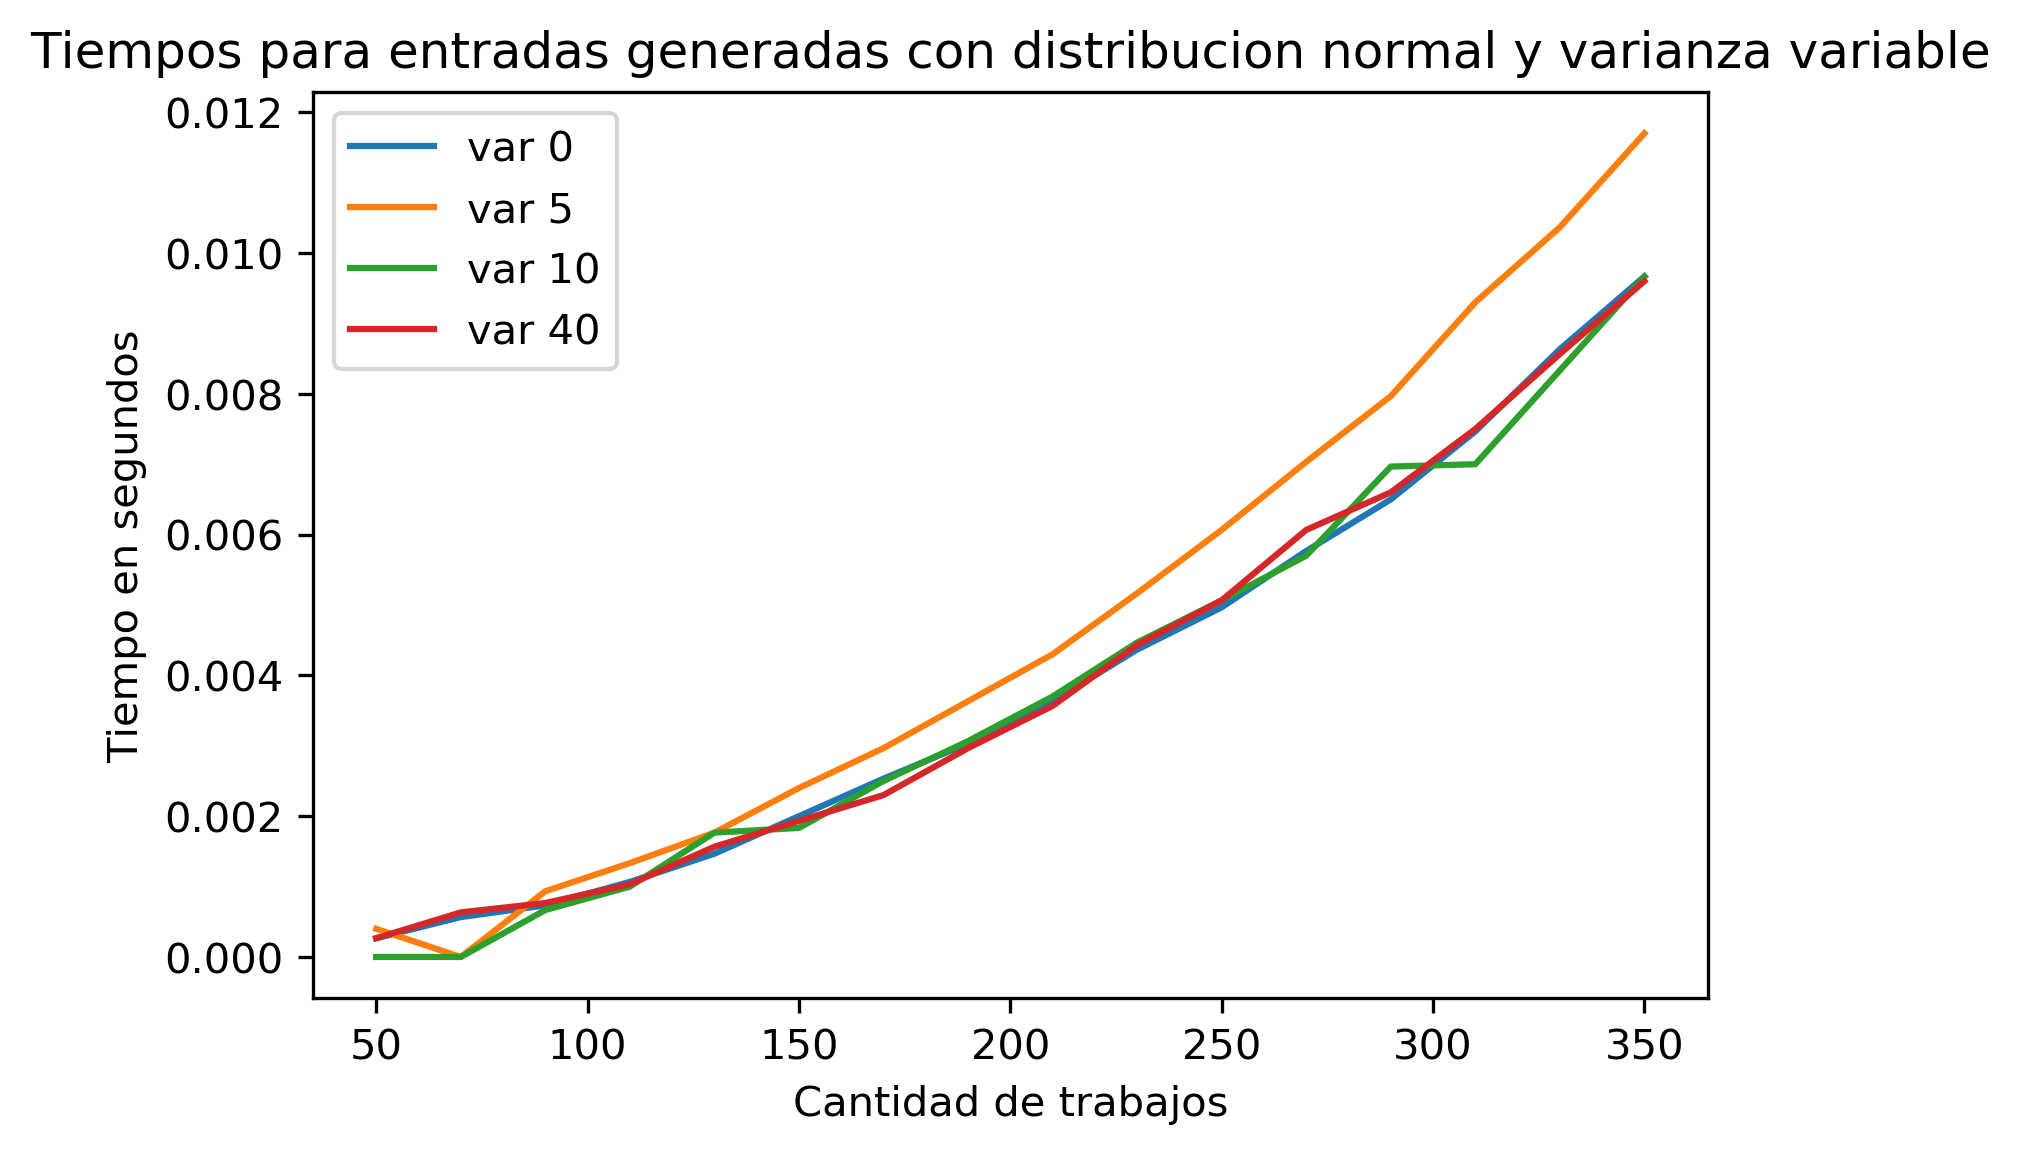
\includegraphics[width=0.6\textwidth]{varianza.png}
    \caption{Tiempo de ejecución en función de \textit{n} con $\mu = 40$ y distintos valores de $\sigma$}
    \label{fig:varianza}
\end{wrapfigure}

Si bien los resultados no son idénticos, son extremadamente similares para todos los tamaños. En todos los casos los tiempos de ejecución se asemejan a una misma función cuadrática. Se decidió terminar la experimentación en una entrada relativamente chica debido a que la generación de tests para casos más grandes eran lentos y ocupaban mucho espacio. Además, los datos obtenidos hasta el momento no indicaban que fuera de alguna utilidad ver más tamaños. La conclusión que podemos sacar de esto es que, como habíamos supuesto, \textbf{la evidencia corrobora} que el tiempo de ejecución va a estar determinado por el \textbf{tamaño de la entrada} y \textbf{no por sus valores}.

\clearpage

\subsection{Experimento 2}

\paragraph{Hipótesis de implementación: } el rendimiento de las implementaciones top down y bottom up no varía significativamente, debido a que las dos necesitan resolver \textbf{todos} los subproblemas de tamaño entre 1 y \textit{n}.

Para comprobar esto no hace falta más que usar los mismos casos de test con ambos algoritmos. El resultado, sin embargo, es más interesante que el de la experimentación anterior. Si bien ambos tiempos de ejecución crecen de forma parecida, la diferencia entre ambos es bastante marcada. 

\begin{wrapfigure}{l}{0.6\textwidth}
    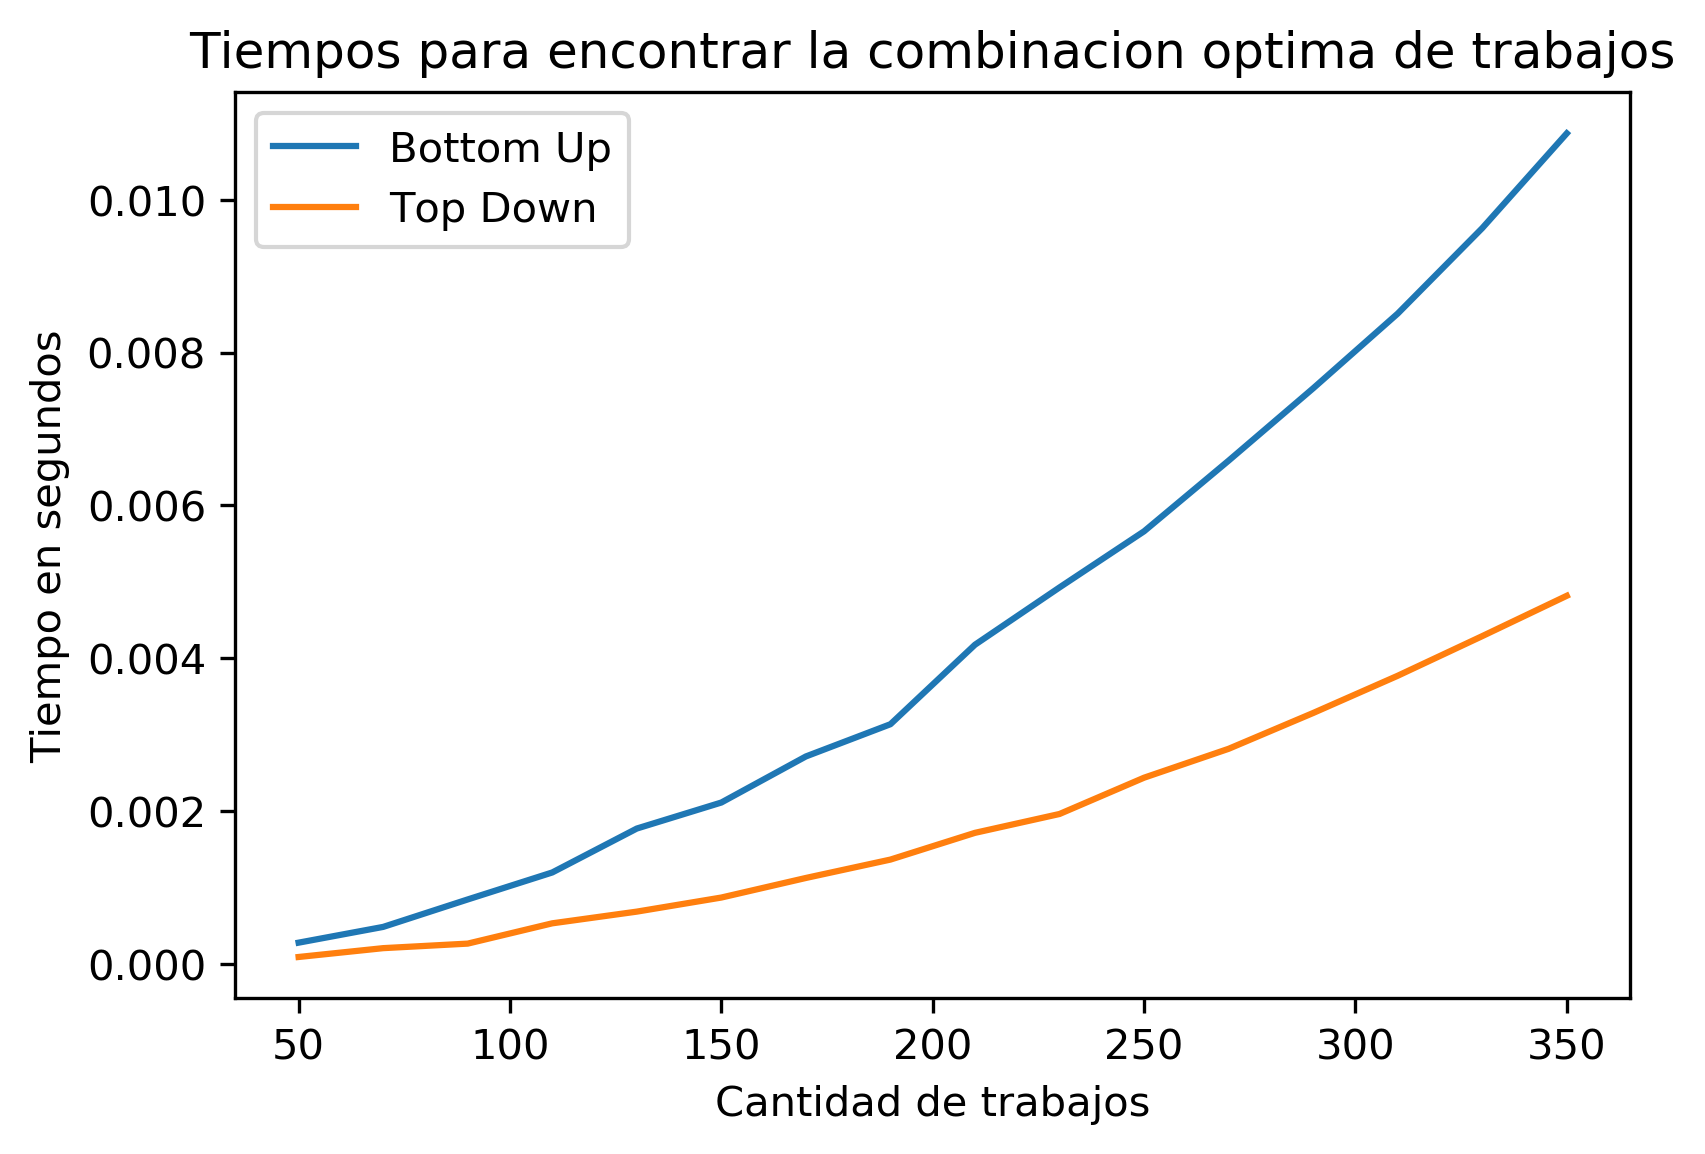
\includegraphics[width=0.6\textwidth]{bottomUp_topDown.png}
    \caption{Tiempo de ejecución para las dos implementaciones}
    \label{fig:bottomup_topdown}
\end{wrapfigure}

Esta vez, si bien ambos gráficos son reminiscentes de funciones cuadráticas, no es una función idéntica compartida para las dos implementaciones; cada una crece a un ritmo distinto. Ya que el análisis algorítmico de ambas implementaciones refleja que la complejidad teórica es la misma, es razonable  La resolución Top Down resultó ser mucho mejor que la Bottom Up que ya de por si es bastante eficiente, llegando a tardar casi la mitad en los casos de mayor tamaño. Inicialmente supusimos que se debía a una diferencia implementativa en cómo reconstruyen la solución, pero al medir el tiempo que tardan solamente en calcular el costo, los resultados observados fueron similares. Esta notable diferencia de resultados \textbf{contradice la hipótesis presentada}. La conclusión que se puede sacar de este experimento es que los resultados empíricos no siempre son predecibles desde lo teórico.

Si bien se visualizan las diferencias entre los tiempos de ejecucion bottom up y top down. Es de esperar que ambos se condigan con los tiempos de ejecución pausibles de un algoritmo cuya complejidad es $\mathcal{O}(n^2)$.
Veamos que esto sucede evaluando la correlación que hay entre los tiempos de ejecución bottom up y una complejidad $\mathcal{O}(n^2)$.


\begin{figure}[h!]
    \begin{subfigure}{0.5\textwidth}
    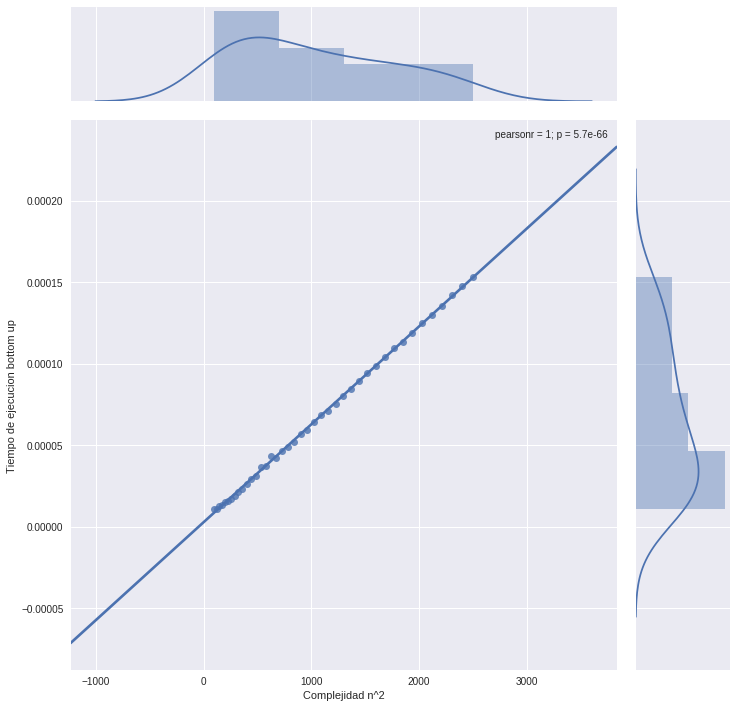
\includegraphics[width=1.0\textwidth]{pearsonBottom.png}
        \caption{Gráfico de correlación para el tiempo de ejecución bottom up y la complejidad $\mathcal{O}(n^2)$}
    \end{subfigure}
    \begin{subfigure}{0.5\textwidth}
        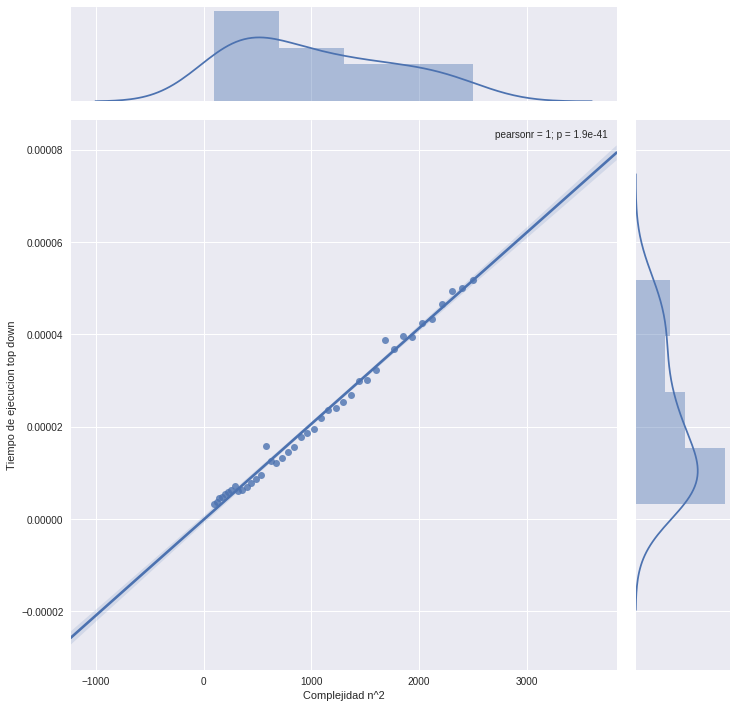
\includegraphics[width=1.0\linewidth]{pearsonTopdown.png}
        \caption{Gráfico de correlación para el tiempo de ejecución top down y la complejidad $\mathcal{O}(n^2)$}    
    \end{subfigure}
\end{figure}


Como se puede observar, en ambos casos obtenemos un coeficiente de correlación lo suficientemente cercano a 1 como para no rechazar la hipótesis de que efectivamente la complejidad $\mathcal{O}(n^2)$ de ambos algoritmos se refleja en la empiria.

\chapter{Problema 2: Replicación de contenido}

\section{Problema a resolver}

\subsection{Descripción}

En este problema contamos con \textit{n} servidores y \textit{m} enlaces que los interconectan; utilizar cada enlace tiene un costo determinado, que es un número entero no negativo. 

En primer lugar queremos hallar un conjunto de enlaces de manera que el costo sea mínimo y la información pueda viajar entre cualquier par de servidores que deseemos. 

Una vez obtenido este conjunto, queremos elegir un servidor \textit{master} desde el que se iniciará la transmisión de la información a todos los otros; nuestro objetivo es que la información tarde lo menos posible en llegar a toda la red. 

Como la información tarda la misma cantidad de tiempo en viajar por cualquier enlace (más allá del costo de usarlo), buscamos un servidor tal que el tiempo máximo que tarda la información en llegar desde él hasta algún otro sea el mínimo posible. 

El problema puede modelarse con un grafo \textit{G} en el que los \textbf{vértices} representan los \textbf{servidores} y las \textbf{aristas} representan los \textbf{enlaces}. A cada arista se le asigna un \textbf{peso} que corresponde al \textbf{costo de usar el enlace}.

Entonces, el primer problema se reduce a encontrar un \textbf{árbol generador mínimo \textit{T}} de \textit{G}. Tiene que ser un árbol generador porque queremos un subgrafo de \textit{G} que contenga todos los vértices y la mínima cantidad necesaria de aristas para que sea conexo; como los costos no pueden ser negativos, sabemos que agregar enlaces \textbf{no puede disminuir el costo total}, por lo que la solución óptima sí o sí será un árbol. Además tiene que ser mínimo porque el peso de las aristas se corresponde con el costo de los enlaces, por lo que encontrar el costo óptimo equivale a \textbf{minimizar el peso del árbol generador}.

El segundo problema a resolver, una vez que tenemos el mínimo árbol generador del grafo, se reduce a hallar un nodo tal que la \textbf{máxima de las distancias} de él a cualquier otro nodo sea la \textbf{minima posible} en todo el grafo.

\subsection{Ejemplo}

Para clarificar consideremos la red dada por el siguiente grafo:

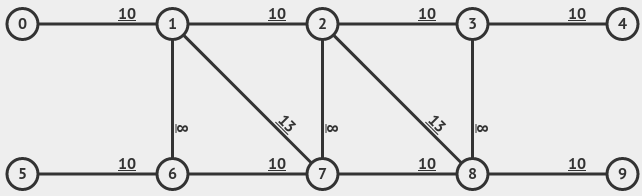
\includegraphics[width=\textwidth]{grafo.png}

Si buscamos la manera de conectar todos los servidores utilizando los enlaces cuyo costo sumado sea el menor posible, daremos con que la solución es la siguiente:

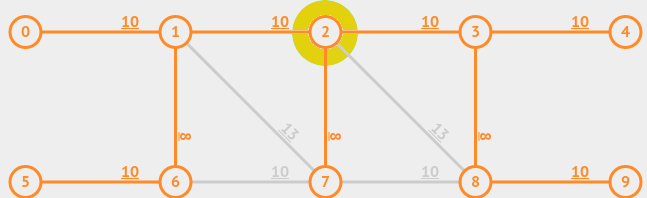
\includegraphics[width=\textwidth]{mst.png}

En esta imagen se pueden ver, coloreados con naranja, los enlaces que minimizan el costo de una conexion entre todos los nodos. 
A la vez, se puede observar marcado con amarillo, el nodo que será utilizado como master.
Este cumple que la maxima distancia que posee hacia otros nodos (hacia 5 y 9 con distancia 3) es la minima entre las distancias maximas de los otros nodos:
el nodo 1 tiene distancia 4 hasta el nodo 9. El nodo 4 tiene distancia 5 hasta el nodo 5, etc....

\section{Parte 1}

\subsection{Algoritmo}
Para conseguir el árbol generador mínimo de un grafo dado, utilizaremos el algoritmo de Kruskal.

\begin{algorithm} \caption{Algoritmo de Kruskal para hallar un árbol generador mínimo}

    \begin{algorithmic}[1]
    
        \Function{generarAGM}{$V, X$} \Comment{V = Nodos, E =  Ejes}
            \State arrayDeEjesDelArbol[]
            \State ordenarPorPeso(X) \Comment{$\mathcal{O}(X log(X))$}
            \For {(u,v) en X} \Comment{$\mathcal{O}(X)$}
                \If {conjuntoAlQuePertenece(u) != conjuntoAlQuePertenece(v)} \Comment{$\mathcal{O}(1)$}
                    \State arrayDeEjesDelArbol.push((u,v))
                    \State unir los conjuntos a los que pertenecen u y v   \Comment{$\mathcal{O}(1)$}
                \EndIf
            \EndFor
        
        \EndFunction
    
    \end{algorithmic}

\end{algorithm}


\subsection{Correctitud}
    El algoritmo de Kruskal es correcto ya que
    \subsubsection{Termina}
    El for-loop externo del algoritmo itera sobre todos los ejes del grafo. Como estamos considerando grafos finitos, entonces el algoritmo termina.
    \subsubsection{La solución es correcta}
    Al ordernar los ejes por peso de menor a mayor, luego irá agregando al árbol los ejes más livianos que puedan formar parte de él. Esto es, que no formen ciclos con los ejes ya elegidos. Como el grafo sobre el que lo llamamos es un grafo conexo, al finalizar nos dará la mayor cantidad de ejes de ese arbol de menor peso que no formen un ciclo. La mayor cantidad posible de ejes que que no formen ciclo sobre un grafo conexo cualquiera es |V| - 1. Como devolvemos un conjunto de ejes que no forman ciclos y tienen cardinal |V| - 1, entonces, por propiedad vista en la práctica, estamos devolviendo un arbol. 
    Como fuimos eligiendo los ejes, ordenados por pesos crecientes, entonces el árbol que devolvemos es mínimo.

\subsection{Complejidad}

El algoritmo de Kruskal tiene complejidad $\mathcal{O}(X log(X))$, que es producto del sort que ocurre en la linea 3. En el peor de los casos la cantidad de ejes \textit{m} es $n(n-1)/2$ de orden $n^2$, lo cual sucede en grafos completos. Por lo cual la complejidad, vista en función de la cantidad de nodos será: $$\mathcal{O}(n^2 log(n^2)) = \mathcal{O}(n^2 2*log(n)) = \mathcal{O}(n^2 log(n))$$

Sin embargo, la parte mas interesante de Kruskal es la que justamente no se refleja en la complejidad final. Sucede en las lineas 5 y 7 del pseudocodigo:

Ambas operaciones fueron marcadas con {$\mathcal{O}(1)$} aunque lograr dicha complejidad en esas operaciones no es trivial. Tras bambalinas se esta utilizando un $disjoint-set$ cuya implementacion permite saber a qué set pertenece un elemento y unir dos sets distintos en $\mathcal{O}(1)$.

Para lograr esto la implementación del $disjoint-set$ se puede realizar utilizando árboles. No indagaremos en profundidad la demostración de la complejidad de este algoritmo ya que excede el scope de este trabajo práctico, pero se puede probar que se condice con la función inversa de Ackermann, que a fines prácticos es $\mathcal{O}(1)$.

\section{Parte 2}

\subsection{Caracterización del nodo master}

Sea \textit{G} un árbol y sean $v_{1}$ y $v_{2}$ los nodos más distantes. Como \textit{G} es un árbol, hay un único camino simple entre cualquier par de nodos, cuya longitud es la distancia entre ellos (debido a esto, a lo largo de esta demostración nos referiremos a la distancia entre dos nodos y a la longitud del camino entre ellos de manera intercambiable). Así $\mathcal{L}(P_{v_{1} v_{2}}) = dist(v_{1}, v_{2})$.

Sea $v$ el punto medio de $P_{v_{1} v_{2}}$, con $\lceil \frac{1}{2} \mathcal{L}(P_{v_{1} v_{2}}) \rceil = max(dist(v,v_{1}), dist(v,v_{2}))$. Queremos probar que \textit{v} es el nodo de \textit{G} cuya distancia máxima a otro nodo es la mínima posible (es decir, es el nodo que minimiza la altura del árbol si es elegido como raíz).

Primero veamos que la máxima distancia de \textit{v} a cualquier otro nodo de \textit{G} es

$$
dmax(v) = \mathcal{L}(P_{v_{1} v_{2}}) = dist(v_{1}, v_{2})
$$

Sea \textit{w} un nodo de \textit{G} y veamos que $dist(v,w) \leq dmax(v)$.

Si $w \in P_{v_{1} v_{2}}$, claramente vale, porque $v_{1}$ y $v_{2}$ son los extremos del camino y puedo extender $P_{vw}$ a $P_{v v_{1}}$ o $P_{v v_{2}}$ según corresponda. Así $d(v,w) = \mathcal{L}(P_{vw}) \leq dmax(v)$.

Si $w \notin P_{v_{1} v_{2}}$, demostremos por el absurdo que $d(v,w) \leq dmax(v)$.

Supongamos que $\mathcal{L}(P_{vw}) = d(v,w) > dmax(v)$ y sea

$$
R = P_{wv} + max\{ P_{v v_{1}}, P_{v v_{2}} \}
$$

Entonces

\begin{align*}
	\mathcal{L}(R) &= \mathcal{L}(P_{wv} + max\{ P_{v v_{1}}, P_{v v_{2}} \}) \\
	&= \mathcal{L}(P_{wv}) + max\{ \mathcal{L}(P_{v v_{1}}), \mathcal{L}(P_{v v_{2}}) \} \\
	&= \mathcal{L}(P_{wv}) + dmax(v) \\
	&> dmax(v) + dmax(v) \\
	&= 2 \times dmax(v) \\
	&= 2 \times \lceil \tfrac{1}{2} \mathcal{L}(P_{v_{1} v_{2}}) \rceil \\
	& \geq 2 \times \tfrac{1}{2} \mathcal{L}(P_{v_{1} v_{2}}) \\
	&= \mathcal{L}(P_{v_{1} v_{2}}) \\
	& \\
	& \therefore \mathcal{L}(R) > \mathcal{L}(P_{v_{1} v_{2}}) \\
\end{align*}


Absurdo, ya que $\mathcal{L}(P_{v_{1} v_{2}})$ es el camino más largo de \textit{G}. El absurdo vino de suponer que $dmax(v)$ no era $\lceil \frac{1}{2} \mathcal{L}(P_{v_{1} v_{2}}) \rceil$.

\medskip

Veamos ahora que no hay ningún nodo cuya distancia máxima a algún otro nodo sea menor a $dmax(v)$.

Sea $u \mid u \neq v \land (\forall w \in V(G)) : d(u,w) < dmax(v) = \lceil \frac{1}{2} \mathcal{L}(P_{v_{1} v_{2}}) \rceil$.

\textit{u} no puede estar en $P_{v_{1} v_{2}}$, ya que si $u \in P_{v_{1} v_{2}} \land u \neq v$, hay un nodo cuya distancia a \textit{u} es mayor a $dmax(v)$:

$$
max \{ d(u,v_{1}), d(u,v_{2}) \} = max \{ \mathcal{L}(P_{u v_{1}}), \mathcal{L}(P_{u v_{2}}) \} > \lceil \tfrac{1}{2} \mathcal{L}(P_{v_{1} v_{2}}) \rceil = dmax(v)
$$

ya que uno de esos dos caminos que parten desde \textit{u} ocupa más de la mitad de $P_{v_{1} v_{2}}$. Entonces $u \notin P_{v_{1} v_{2}}$.

Como $u \neq v$, hay un camino simple único $P_{uv}$, con $\mathcal{L}(P_{uv} > 0$.

Sea $R' = max \{ P_{u v_{1}}, P_{u v_{2}} \}$. Como \textit{u} es tal que $(\forall w \in V(G)) : d(u,w) < dmax(v)$, debería valer

$$
\mathcal{L}(R') = max\{ d(u,v_{1}), d(u,v_{2}) \} < dmax(v)
$$

Pero

\begin{align*}
    \mathcal{L}(R') &= \mathcal{L}( max \{ P_{u v_{1}}, P_{u v_{2}} \} ) \\
    &= \mathcal{L}( max \{ P_{uv} + P_{v v_{1}}, P_{uv} + P_{v v_{2}} \} ) \\
    &= max \{ \mathcal{L}(P_{uv}) + \mathcal{L}(P_{v v_{1}}), \mathcal{L}(P_{uv}) + \mathcal{L}(P_{v v_{2}}) \} \\
    &= \mathcal{L}(P_{uv}) + max \{ \mathcal{L}(P_{v v_{1}}), \mathcal{L}(P_{v v_{2}}) \} \\
    &> max \{ \mathcal{L}(P_{v v_{1}}), \mathcal{L}(P_{v v_{2}}) \} \\
    &= dmax(v) \\
    & \\
    & \therefore \mathcal{L}(R') > dmax(v) \\
\end{align*}

Absurdo.

El absurdo vino de suponer que \textit{v} no era el nodo de \textit{G} cuya distancia máxima a otro nodo era la mínima posible.

\paragraph{Observación:} $v_{1}$ y $v_{2}$ seguro son hojas. Si no lo fueran, podríamos extender el camino entre ellos con más nodos y no sería el más largo.

\subsection{Algoritmo}

\subsubsection{Pseudocódigo}
Veamos ahora el pseudocódigo para la segunda parte del problema, la de encontrar el nodo máster: 
\begin{algorithm}[H] \caption{Encontrar raiz del árbol}

    \begin{algorithmic}[1]
    
        \Function{encontrarRaiz}{$V, X$} \Comment{V = Nodos, E = Ejes del árbol}
            
            \State nodoInicial $\rightarrow$ 1
            \State distanciasAOtrosNodos = conseguirDistanciasDesde(nodoInicial) \Comment{BFS, $\mathcal{O}(n)$}
            \State primeraHojaDelCaminoMasLargo = max(distanciasAOtrosNodos) \Comment{búsqueda lineal de máximo, $\mathcal{O}(n)$}
            \State distanciasAOtrosNodos = 
            DistanciasDesde(primeraHojaDelCaminoMasLargo) \Comment{Segundo BFS, $\mathcal{O}(n)$}
            \State segundaHojaDelCaminoMasLargo = max(distanciasAOtrosNodos) \Comment{búsqueda lineal de máximo, $\mathcal{O}(n)$}
            \State caminoMasLargo = conseguirCamino(primeraHojaDelCaminoMasLargo,segundaHojaDelCaminoMasLargo) \Comment{BFS que reconstruye el camino guardándose el nodo previo, $\mathcal{O}(n)$}
            \State raiz = caminoMasLargo[|caminoMasLargo| / 2]
            \State \Return raiz
        \EndFunction

    
    \end{algorithmic}

\end{algorithm}

\subsection{Correctitud}

Veamos que el nodo encontrado en el primer BFS es uno de los extremos del camino simple más largo.

Para empezar, consideremos que el grafo de entrada es un árbol, por lo que \textbf{hay un único camino simple entre cualquier par de vértices}. Como BFS devuelve los caminos mínimos (que sí o sí son simples) desde un nodo a todos los demás en un grafo sin pesos, se deduce que si lo ejecutamos en un árbol, alguno de los caminos devueltos es el máximo camino simple posible, puesto que son únicos.

Sea \textit{w} un nodo cualquiera de \textit{G} y sea \textit{w'} el nodo más lejano a \textit{w}. Queremos probar que o bien $w' = v_{1}$ o $w' = v_{2}$.

Si $w = v_{1}$ o $w = v_{2}$, trivialmente $w' = v_{1}$ o $w' = v_{2}$, porque tiene que ser el otro extremo del camino más largo.

Si $w \neq v_{1}$ y $w \neq v_{2}$, supongamos que $w' \neq v_{1}$ y $w' \neq v_{2}$ y lleguemos a un absurdo. Como BFS recorre todos los nodos de \textit{G}, en algún punto de la búsqueda llega a un nodo $v' \in P_{v_{1} v_{2}}$.

Puesto que $w' \neq v_{1}$ y $w' \neq v_{2}$, hay al menos tres caminos distintos que empiezan en \textit{v'}: $P_{v'w'}, P_{v' v_{1}} y P_{v' v_{2}}$. Como \textit{w'} es el nodo de mayor distancia a \textit{w}, tiene que valer que $\mathcal{L}(P_{v'w'}) > max\{ \mathcal{L}(P_{v' v_{1}}), \mathcal{L}(P_{v' v_{2}}) \}$, pues de lo contrario el algoritmo habría elegido a $v_{1}$ o a $v_{2}$ en vez de elegir a \textit{w'}. Entonces vale que

\begin{align*}
    \mathcal{L}(P_{v_{1} w'}) &= \mathcal{L}(P_{v_{1} v'} + P_{v'w'}) \\
    &= \mathcal{L}(P_{v_{1} v'}) + \mathcal{L}(P_{v'w'}) \\
    &> \mathcal{L}(P_{v_{1} v'}) + \mathcal{L}(P_{v' v_{2}}) \\
    &= \mathcal{L}(P_{v_{1} v'} + P_{v' v_{2}}) \\
    &= \mathcal{L}(P_{v_{1} v_{2}}) \\
    & \\
    & \therefore \mathcal{L}(P_{v_{1} w'}) > \mathcal{L}(P_{v_{1} v_{2}}) \\
\end{align*}

Absurdo, ya que habíamos supuesto que $P_{v_{1} v_{2}}$ era el camino más largo. El absurdo vino de suponer que \textit{w'} no era $v_{1}$ ni $v_{2}$.

Entonces, como \textit{w'} es uno de los extremos del camino más largo, el segundo BFS va a elegir el otro extremo, por lo que el algoritmo es correcto.

\subsection{Complejidad}

Encontrar el nodo master entonces depende de encontrar el camino más largo en el grafo. 
Para ello, realizamos dos busquedas BFS sobre un arbol. En la primera, encontramos la primer hoja del camino mas largo y en la segunda, la otra hoja. 

La complejidad de BFS es $\mathcal{O}(|V| + |E|)$ (recordemos que $n = |V|$ y $m = |E|$). Sin embargo como lo estamos efectuando sobre un arbol donde $|E| = |V| - 1$ entonces la complejidad de cada BFS es $\mathcal{O}(|V|)$.

Una vez que damos con las dos hojas del camino más largo, buscamos el camino entre ellas. Esto también lo podemos hacer con BFS: lo llamamos desde una de las hojas del camino mas largo y guardamos en un nuevo array en la posicion de cada nodo quién fue el nodo previo. Como es BFS sobre un arbol es $\mathcal{O}(|V|)$.

Una vez que contamos con el nodo previo para cada nodo respecto del camino que lleva desde una hoja del camino más largo hacia él, se puede reconstruir el camino más largo de todo el grafo del siguiente modo: nos posicionamos en la otra hoja del camino más largo (sobre la que no llamamos a BFS) y pedimos su nodo previo. Luego vamos a dicho nodo y pedimos su nodo previo y así sucesivamente. Si repetimos este proceso, eventualmente llegaremos a la hoja del camino más largo sobre la que llamamos a BFS. Una vez que damos con ella, terminamos el procedimiento.

A lo sumo el camino más largo tiene $|V|$ nodos y encontrar el nodo previo de a cada nodo era $\mathcal{O}(1)$, ya que nos habíamos creado un array donde consultar dicha información. 

Por tanto la complejidad resultante de este procedimiento es $\mathcal{O}(|V|)$ * $\mathcal{O}(|1|)$ = $\mathcal{O}(|V|)$.

\section{Experimentación}

A continuación presentamos la experimentación para las dos partes del problema.

\subsection{Generación de casos de test}

Cada caso de test fue generado con un script de Python que toma como parámetros la cantidad de nodos \textit{n}, la media $\mu$, la varianza $\sigma$ y un número de punto flotante $p_{b}$ entre 0 y 1 (inclusive). Los pesos de las aristas siguen una distribución $N(\mu, \sigma)$. $p_{b}$ tiene la función de ajustar la \textbf{cantidad esperada de aristas del grafo}. Como es precondición que el grafo sea conexo, el script inicialmente genera un grafo completo, lo recorre con DFS, busca todos los \textit{backedges} -aristas tales que el grafo \textbf{sigue siendo conexo} si se las saca- y elimina cada una independientemente de todas las otras con una probabilidad $1 - p_{b}$. Entonces, si $p_{b}$ es 0, el resultado es un grafo sin \textit{backedges}, es decir un árbol de DFS; si es 1, es un grafo completo. Por la forma en que son elegidas las aristas a eliminar, \textbf{siempre es conexo}.

En general, como el grafo inicialmente tiene $n (n-1) / 2$ aristas, la mínima cantidad que puede tener es $n-1$ (porque en ese caso es un árbol, y los árboles son minimales con respecto a ser conexos) y la máxima es $n (n-1) / 2$. Además, si un grafo completo tiene $n (n-1) / 2$ aristas y $n-1$ de ellas forman parte del árbol de DFS, debe tener $n (n-1) / 2 - (n-1) = (n-1) (n-2) / 2$ \textit{backedges}. Entonces, el valor esperado de \textit{m} para un grafo generado con este script es

$$
E(m) = n-1 + p_{b} (n-1) (n-2) / 2
$$

\subsection{Experimento 3}

En el análisis del primer algoritmo (Kruskal), podemos ver que su complejidad está dominada por un \textit{sort} de orden $\tilde{O}(m log(m))$ que ordena las aristas crecientemente según su peso. Según la documentación de la librería \textit{standard} de C++11, que se usó para implementar este algoritmo, esa es la complejidad del sort en el peor caso \footnote{http://en.cppreference.com/w/cpp/algorithm/sort}. En un algoritmo de estas características, no es esperable que el tiempo de ejecución varíe según los valores de los elementos de una entrada, sólo que aumente según el tamaño del vector a ordenar. Sin embargo, para grafos con una cantidad de vértices determinada, sí es esperable que el tiempo de ejecución empeore en función de la cantidad de aristas (la \textit{densidad}). Es así que desarrollamos esta hipótesis:

\paragraph{Hipótesis de densidad: } para los mismos valores de la cantidad de vértices \textit{n}, el tiempo de ejecución del algoritmo de Kruskal aumenta en función de la cantidad de aristas \textit{m}.

Para ver esto, realizamos una prueba variando $p_{b}$ para valores desde 0 (árboles) hasta 1 (grafos completos), con intervalos de 0.25. Para cada una de estas variantes, corrimos 200 experimentos y tomamos la media entre ellos. El resultado de la experimentación puede verse en la figura \ref{fig:tiemposmst}.

\begin{figure}[h]
    \centering
    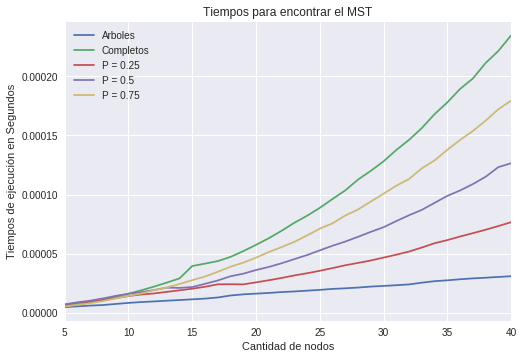
\includegraphics[width=0.75\textwidth]{tiempoDeMst.png}
    \caption{Tiempo de ejecución del algoritmo 1}
    \label{fig:tiemposmst}
\end{figure}

\paragraph{Observaciones: } a medida que la cantidad de ejes esperada es mayor para cada grafo, aumentan los tiempos de ejecución. Es así como los árboles tienen los menores tiempos de ejecución, mientras que los completos tienen los mayores. A la vez se puede visualizar que los tiempos de ejecución a mayor cantidad de ejes se asemejan a una función cuadrática, mientras que los de árboles parecen más bien cuasi-lineales. Los siguientes experimentos se hicieron con el fin de corroborar estas últmas afirmaciones.

\subsection{Experimento 3 bis}

\paragraph{Contrastación de la complejidad teórica en la empiria: } El tiempo de ejecución del algoritmo de Kruskal para grafos completos es $\mathcal{O}(n^2log(n))$.

\medskip

Realizamos un diagrama de Pearson contrastando los tiempos de ejecución de los grafos completos de n nodos con la funcion $n^2log(n)$. Se lo puede ver en la figura \ref{fig:pearsonN2logN} de la página siguiente.

\newpage

\begin{figure}[h!]
    \centering
    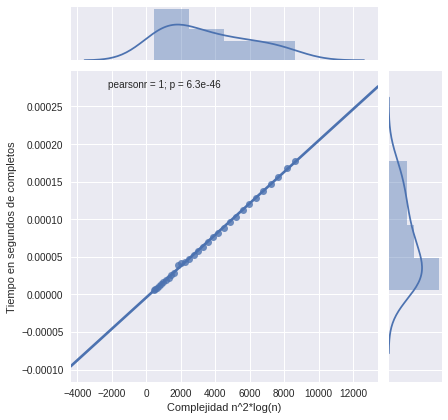
\includegraphics[width=0.65\textwidth]{pearsonCompleteN2LOGN.png}
    \caption{Semejanza entre los tiempos de ejecución del algoritmo 1 y la función $n^2 log(n)$.}
    \label{fig:pearsonN2logN}
\end{figure}

\paragraph{Observaciones:} El coeficiente de Pearson es 1 con un p-value suficientemente pequeño como para \textbf{no poder rechazar la hipótesis} de que la complejidad teórica se condice con los resultados empíricos.

\medskip

¿Sucederá lo mismo para los grafos que eran árboles? Como el sort de Kruskal se realiza sobre todas los ejes y en ese caso la cantidad de ejes no era $\mathcal{O}(n^2)$ sino $\mathcal{O}(n)$, entonces lo esperable es que la complejidad no sea similar a $\mathcal{O}(n^2log(n))$ sino más bien $\mathcal{O}(nlog(n))$.

Veamos el diagrama de Pearson para estas complejidades y los tiempos de ejecución en árboles:

\begin{figure}[h!]
    \begin{subfigure}{0.5\textwidth}
        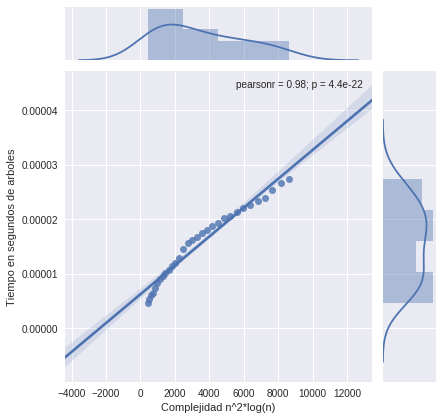
\includegraphics[width=1.0\linewidth]{pearsonTreeN2LOGN.png}
        \caption{Grafos completos}
    \end{subfigure}
    \begin{subfigure}{0.5\textwidth}
        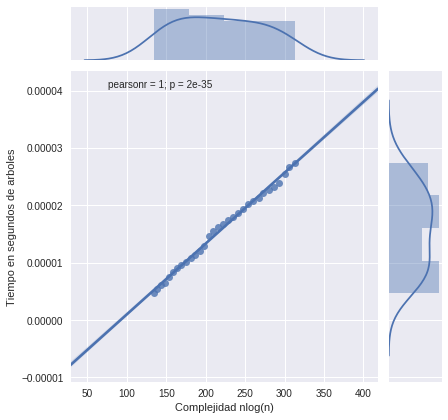
\includegraphics[width=1.0\linewidth]{pearsonTreeNLOGN.png}
        \caption{Árboles}
    \end{subfigure}
    \caption{Similitud entre la complejidad empírica y la teórica para grafos con distintas densidades}
    \label{fig:pearsontrees}
\end{figure}


Como se puede ver, para árboles, los tiempos de ejecución se asimilan más bien a una complejidad $\mathcal{O}(nlog(n)$, lo cual se condice con lo que supusimos. Como el sort de los ejes domina la complejidad de Kruskal, variar la cantidad de ejes sobre los que se hace el sort hace variar la complejidad teórica y esto se refleja en la empiria.

\subsection{Experimento 4}

Una cosa que observamos durante el desarrollo del segundo algoritmo para este problema es que \textbf{siempre} va a tener que pasar por todas las aristas del árbol generador dos veces, puesto que BFS (según fue visto en clase) recorre todas las aristas. Más allá de las características particulares del árbol (si es un camino, si al elegir una raíz es un árbol \textit{k}-ario para cierto \textit{k}, etc.) el algoritmo va a mirar las $n-1$ aristas. En un principio, conjeturamos que el algoritmo debería tardar prácticamente lo mismo en cualquier árbol con un número de aristas fijo, más allá de su topología. Sin embargo, después de analizar con mayor detenimiento la búsqueda del nodo master, notamos que debe reconstruir el camino más largo para poder devolverlo. Sería esperable, entonces, que el tiempo de ejecución \textbf{aumente} para árboles de \textbf{mayor diámetro} \footnote{El diámetro se define como la mayor distancia entre un par de vértices cualesquiera de un grafo.}.

\paragraph{Hipótesis del camino más largo: } para árboles con una misma cantidad de nodos \textit{n}, el tiempo de ejecución del algoritmo aumenta en función de su diámetro \textit{d}, ya que la búsqueda del nodo master es de orden $\mathcal{O}(d)$.

\medskip

Si esta hipótesis es verdadera, deberíamos ver que el tiempo de ejecución aumenta \textbf{linealmente} en función de la altura, y que la cantidad total de vértices actúa como una constante aditiva.

Experimentalmente, calculamos el tiempo de ejecución para entradas de 20 a 100 nodos, con intervalos de a 20 nodos. Luego dentro cada entrada con una cantidad de nodos, fue variando la longitud del camino más largo. En cada caso esta iba desde 2 hasta $n-1$. 

Para cada una de estas combinaciones se tomó la media de 50 ejemplos. Los resultados son los siguientes:

\begin{figure}[h!]
    \centering
    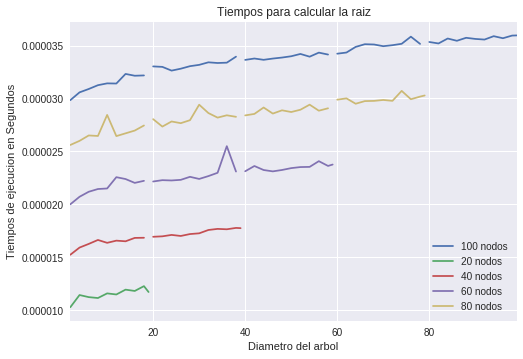
\includegraphics[width=0.75\textwidth]{tiempoRaizDeArboles.png}
    \caption{Tiempo de ejecución del algoritmo 2 para árboles de distintos diámetros}
    \label{fig:tiempoarboles}
\end{figure}

Como se puede observar, al incrementar la cantidad total de nodos se incrementa un costo base para cada caso. Es de suponer que esto se deba a que el algoritmo BFS necesario para encontrar las hojas del camino mas largo tardará más a medida que haya mayor cantidad de nodos. Es interesante notar que para este conjunto de casos de test, \textit{n} actuó como una constante aditiva, puesto que todos los gráficos tienen una pendiente casi igual pero su ordenada al origen es distinta.

A la vez, dentro de los casos para un numero de nodos fijo, vemos que en árboles de mayor diámetro, el tiempo de ejecución aumenta. Esto sucede en todos los casos sin importar la cantidad total de nodos. Por lo tanto, el experimento brinda \textbf{evidencia a favor de la hipótesis}.

Cabe ahora estudiar cómo es que aumenta el tiempo de ejecución del calculo del nodo raiz/master.

En teoría, para encontrar el nodo master realizamos dos BFS que tienen complejidad $\mathcal{O}(n)$ cada uno por ser ejecutados sobre un árbol y luego reconstruimos el camino más largo también en $\mathcal{O}(n)$ (con una cota más ajustada $\mathcal{O}(d)$ por lo argumentado más arriba; es fácil ver que \textit{d} está acotado por \textit{n}). Sería entonces de esperar que haya una alta correlación entre los tiempos de ejecución para encontrar la raíz variando la cantidad de nodos y la complejidad $\mathcal{O}(n)$.

Realizamos un experimento en donde comprobamos esto y el diagrama de Pearson es el siguiente:

\begin{figure}[h!]
    \centering
    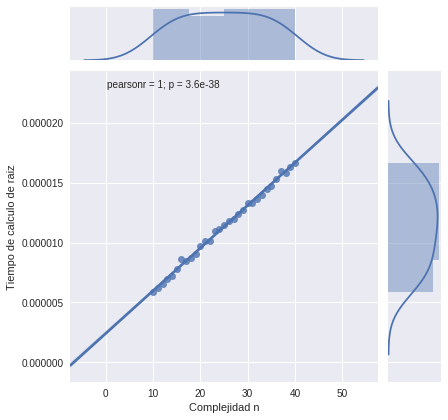
\includegraphics[width=0.65\textwidth]{pearsonCalculoRaiz.png}
    \caption{Caption}
    \label{fig:pearsonraiz}
\end{figure}

En efecto se puede verificar con alto grado de confianza que la suposición teórica de que el calculo de la raiz se realiza con complejidad $\mathcal{O}(n)$ se refleja también en los tiempos de ejecución del algoritmo.

\chapter{Problema 3: Transportes pesados}

\section{Problema a resolver}

\subsection{Descripción}

Queremos abastecer a \textit{C} clientes con ladrillos, los cuales salen de cualquiera de las \textit{F} fábricas. En principio, disponemos de \textit{R} rutas que unen indistintamente fábricas y clientes para hacer las entregas. Como nuestros ladrillos no son huecos, los cargamentos resultan demasiado pesados para las rutas, y se nos ha informado que no podremos seguir usándolas sin antes hacer una inversión para reforzarlas \footnote{http://bit.ly/2hE4oDN}. Sin embargo, hacer estas obras es costoso y deberemos escoger cuidadosamente las rutas a mejorar. Nuestro objetivo es minimizar los costos de las obras sin dejar de abastecer a ningún cliente. Es decir, queremos encontrar el conjunto de caminos que nos permita llegar a cada cliente y mantenga el costo total de las obras lo más bajo posible. El costo de arreglar una ruta es proporcional a su longitud, por lo que, para mantener los gastos bajos, deberíamos encontrar los caminos de menor longitud (en total) que nos permitan llegar a los destinos. Es importante destacar que no buscamos conseguir el camino mínimo desde una fábrica hasta cada cliente en particular, sino un conjunto de caminos que nos permita llegar hasta cada cliente desde al menos una fábrica y tenga distancia mínima total.

Dada nuestra intención de poder llegar desde todo cliente hasta alguna fábrica, podemos modelar la solución como un grafo en el que todo nodo cliente tenga un camino a algún nodo fábrica. Esto nos lleva a pensar que la solución va a ser un árbol generador de \textit{G}, ya que todos los nodos deberían estar incluidos y debe haber caminos entre los nodos, y además debe ser mínimo para optimizar el costo. No obstante, esta solución no es del todo óptima en todos los casos, podría suceder que tenga rutas extra: quizás tenga aristas que unen fábricas con fábricas, lo cual no me aportaría nada, y además tendría camino desde cada cliente a más de una fábrica, lo cual es innecesario ya que con que pueda llegar desde una alcanza. Entonces a este árbol generador minimo del grafo podríamos sacarle algunas aristas (las que unen fábricas y las que unen clientes con fábricas con caminos peores a otros existentes) y las fábricas redundantes, si las hubiera, y así mejorar nuestra solución. El resultado de esto es un bosque, donde cada árbol tiene exactamente una fábrica y al menos un cliente, cada uno de los clientes está en alguna componente conexa, y además la suma de los pesos de cada árbol es óptima. Puede ocurrir que no todas las fábricas están en la solución.

El problema puede modelarse con un grafo \textit{G} en el que los \textbf{vértices} representan tanto los \textbf{clientes} como las \textbf{fábricas} y las \textbf{aristas} representan las \textbf{rutas}. A cada arista se le asigna un \textbf{peso} que corresponde a su longitud. La solución será $G_r = (V_r, X_r)$, un subgrafo de \textit{G} donde las aristas representan las rutas que se reforzarán y los vértices son todos los clientes y fábricas conectados por ellas.

\subsection{Formalización}

Dada esta descripción podemos comenzar a enumerar las características de nuestro grafo:

\begin{equation} 
    V_r \textit{ necesariamente contiene al conjunto } C
\end{equation}

El problema requiere que todos los clientes sean conectados con al menos una fábrica. Es evidente que nuestra solución deberá contenerlos a todos.

\begin{equation} 
    \textit{La solución no es necesariamente conexa}
\end{equation}

Aún si el grafo de entrada $G$ es conexo, la solución $G_r$ no necesariamente lo es. Lo único que sabemos es que como $G_r$ es subgrafo de $G$, $G$ no conexo implica $G_r$ no conexo.

Se puede pensar un caso sencillo donde hay dos clientes y dos fábricas: cada cliente está cerca de una fábrica, pero los clientes y las fábricas están lejos entre sí. La solución entonces es un grafo con las aristas $\{(c_1, f_1), (c_2, f_2)\}$ conectando a cada cliente con su fábrica más cercana, donde existen dos componentes conexas $CC_1 = \{c_1, f_1\}$ y $CC_2 = \{c_2, f_2\}$. Cabe mencionar que de existir una única fábrica todos los clientes deberán ser atendidos por ella, y la solución será conexa.

\begin{equation} 
    X_r \textit{ no necesariamente contiene a todo el conjunto } F
\end{equation}

Imaginemos nuevamente un ejemplo sencillo para explicar esto: la fábrica $f_1$ está conectada únicamente a la fábrica $f_2$, que a su vez está conectada a los clientes $c_1$ y $c_2$. Necesariamente incluiremos en la solución las aristas $\{(c_1, f_2), (c_2, f_2)\}$, ya que de no ser así estos clientes no estarán abastecidos. Pero al hacer esto encontramos la (única) solución al problema, ya que ahora todos los clientes están conectados con una fábrica a través de una ruta reforzada. Vemos que la fábrica $f_1$ no forma parte de la solución.

\begin{equation}
    \textit{Las componentes conexas de la solución con más de un vértice tienen al menos un cliente y una fábrica}
\end{equation}

Sean $CC_f$ las componentes conexas de la solución que contienen fábricas.
Por definición, $G_r$ contiene a todos los clientes y las fábricas conectadas por ellos.
Por lo tanto para toda fábrica existe al menos un cliente con la que está conectada.
Por lo tanto para cada $CC_f$, habrá al menos un cliente y una fábrica.

Queremos ver ahora que no existen las componentes conexas $CC_{nf}$ que no contienen fábricas.
Supongamos por absurdo que existe $CC \in CC_{nf}$.
Entonces $CC$ contiene al menos un cliente $c$, ya que si no, no sería un grafo.
Pero esto es absurdo ya que de ser así el cliente $c$ no tendría camino a ninguna fábrica y quedaría desabastecido.

Entonces todas las componentes conexas de la solución contienen al menos una fábrica, y también tienen al menos un cliente por definición de la solución.

\begin{equation} 
    \textit{Las componentes conexas de la solución son árboles}
\end{equation}

Sea $CC$ una componente conexa de la solución. $CC$ es una subsolución de peso mínimo que incluye a todos sus vértices.
Queremos suponer por absurdo que $CC$ no es un árbol.
$CC$ conexo y no árbol $\implies$ $CC$ tiene al menos un ciclo, al que llamaremos $L$.
Existe entonces una arista $e \in L$ tal que si la remuevo $CC - e$ sigue siendo conexo.
Para todo par de vértices en $CC - e$ sigue existiendo un camino que los une, y por lo tanto $CC - e$ también es subsolución para su conjunto de vértices.
Pero todas las aristas tienen peso positivo, y entonces $peso(CC - e) < peso(CC)$ \textbf{ABS}.
El absurdo viene de suponer que $CC$ no era un árbol $\square$.

\begin{equation}
    \textit{Las componentes conexas de la solución tienen una única fábrica}
\end{equation}

Sea $CC$ una componente conexa de la solución.
Sabemos que $CC$ contiene al menos una fábrica $f_1$.
Queremos suponer por absurdo que existe más de una fábrica en $CC$.
Sabemos que $CC$ es un árbol $\implies$ existe un único camino entre todo par de vértices.
Entonces existe una fábrica $f_2$ y existe un cliente $c$, y hay un único camino $P$ que une a los tres.
Se pueden dar tres posibilidades:

\begin{enumerate}  
\item $P = \{c,...,f_1,...,f_2\}$
\item $P = \{f_1,...,c,...,f_2\}$
\item $P = \{f_1,...,f_2,...,c\}$
\end{enumerate}

Para el caso 1, existe una arista $e = (e_1, e_2)$ en $P_{f_1 \rightarrow f_2}$ tal que si la remuevo, todos los vértices en $P_{c \rightarrow e_1}$ siguen conectados a al menos una fábrica ($f_1$). También, todos los vértices en $P_{e_2 \rightarrow f_2}$ siguen conectados a al menos una fábrica ($f_2$).

Para el caso 2: existe una arista $e = (e_1, c)$ en $P_{f_1 \rightarrow c}$ tal que si la remuevo, todos los vértices en $P_{f_1 \rightarrow e_1}$ siguen conectados a al menos una fábrica ($f_1$). También, todos los vértices en $P_{c \rightarrow f_2}$ siguen conectados a al menos una fábrica ($f_2$).

El caso 3 es análogo al caso 1, intercambiando las etiquetas de las aristas $f_1$ y $f_2$.

En los tres casos, todo vértice en $CC - e$ o bien es una fábrica o bien tiene al menos un camino que lo une a una fábrica, y por lo tanto $CC - e$ también es subsolución para su conjunto de vértices.
Pero todas las aristas tienen peso positivo, y entonces $peso(CC - e) < peso(CC)$ \textbf{ABS}.
El absurdo viene de suponer que existe más de una fábrica en $CC$ $\square$.

\newpage

\subsection{Ejemplo}

Veamos un caso en el que la empresa tiene fábricas en Buenos Aires, Mar del Plata, Necochea y Tandil:

\begin{center}
    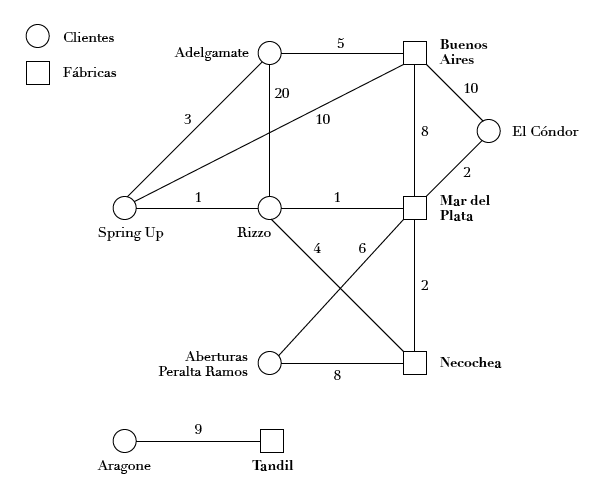
\includegraphics[width=0.6\textwidth]{elcondor-01.png}
\end{center}

Como podemos ver, el grafo de entrada no es conexo, por lo que hay pares de nodos entre los que no hay caminos. Sin embargo, sí se verifica que \textbf{desde cualquier cliente hay un camino a alguna fábrica}.

\begin{center}
    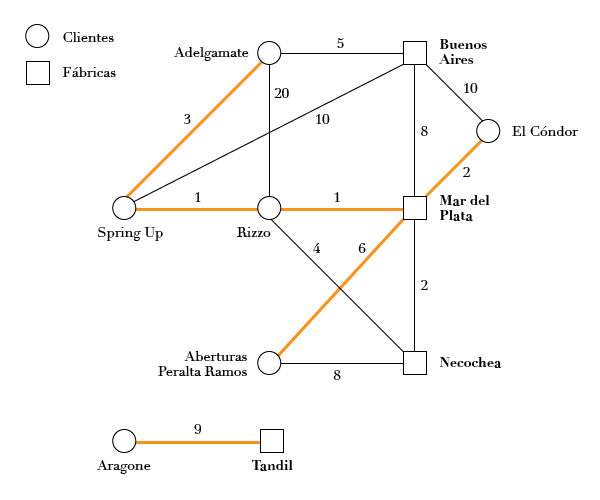
\includegraphics[width=0.6\textwidth]{elcondor-02.png}
\end{center}

Las aristas marcadas en naranja representan la selección óptima de rutas. La solución es un bosque, es disconexa (en otros grafos podría ser conexa), no tiene ninguna componente conexa con más de dos fábricas y todas sus componentes conexas con más de un vértice contienen una fábrica y al menos un cliente.

\section{Algoritmo y correctitud}

El algoritmo que genera la solución utiliza la idea del algoritmo de Kruskal. Al igual que Kruskal, ordenamos las aristas por peso, de menor a mayor, y luego las vamos recorriendo, agregándolas o no a nuestro bosque. La diferencia está en que en cada arista, además de ver que no genere ciclos en el grafo que estamos armando, también vemos que no una dos componentes conexas que ya tengan fábricas.
Esto nos asegura que en cada componente conexa quede solo una fábrica. El resultado va a ser un bosque en el que todo cliente esté conectado a una fábrica de forma tal que el peso total de cada árbol es el mejor posible. Esto sucede dado que agregamos las aristas de forma ordenada. Siempre voy a ver primero las de menor peso, entonces no puede pasar que en algún momento encuentre una arista que me convenía más que alguna que ya puse, entonces la solución es la mejor.

Como fue demostrado, la solución es un conjunto de componentes conexas que son árboles que contienen una única fábrica. El algoritmo propuesto se basa, al igual que Kruskal, en unir conjuntos usando aristas de peso mínimo. Únicamente se evita agregar aristas cuando conecten dos conjuntos en los que ambos hayan fábricas.

¡Con esta sencilla modificación al Algoritmo de Kruskal logramos obtener una solución al problema!

Veamos que se cumplen el resto de las propiedades:

\begin{enumerate}
    \item \textit{La solución es mínima}: se desprende de la demostración del Algoritmo de Kruskal, ya que nuestro algoritmo es igual salvo por la restricción de agregar caminos entre fábricas.
    \item \textit{Las componentes conexas de la solución son árboles}: se desprende del invariante del Algoritmo de Kruskal.
    \item \textit{Las componentes conexas de la solución tienen al menos un cliente y una fábrica}: se cumple dado que por especificación todos los clientes tienen al menos un camino a una fábrica, y se unirán vértices mientras haya al menos una componente conexas sin fábricas.
\end{enumerate}

\subsection{Pseudocódigo}

\begin{algorithm} \caption{Mínimo subgrafo tal que hay un camino desde cualquier cliente a una fábrica}

    \begin{algorithmic}[1]
    
        \Function{MinimoSubgrafo}{$C, F, rutas$}
        \Comment{C = \#clientes, F = \#fábricas, rutas = lista de rutas}
            
            \State ordenarPorPeso(rutas) \Comment{$\mathcal{O}(R log(R))$}
            \State $conjuntos \leftarrow \{1,...C,C+1,..,F\}$
            \State $T \leftarrow \emptyset$
            
            \For{$r \in$ rutas} \Comment{$\mathcal{O}(R)$}
                \If{$r$ no une dos conjuntos con fábricas y no forma ciclos}
                    \State unir los conjuntos a los que pertenecen $\pi_{1}(r)$ y $\pi_{2}(r)$
                    \State $T \leftarrow T \cup \{ r \}$
                \EndIf
            \EndFor
        
        \EndFunction
    
    \end{algorithmic}

\end{algorithm}

\section{Complejidad}

Como podemos ver en los comentarios del pseudocódigo, la complejidad del algoritmo es

$$
\mathcal{O}(R log(R)) + \mathcal{O}(r) = \mathcal{O}(R log(R))
$$

pero la complejidad pedida es $\mathcal{O}(R log(C))$. Veamos que en un problema de estas características, las dos complejidades son equivalentes.

Como \textit{R} es la \textbf{cantidad de aristas del grafo}, no puede exceder $(F+C)(F+C-1)/2$, por lo que \textit{R} es de orden $\mathcal{O}((F+C)^2)$. Esta relación entre vértices y aristas vale para grafos en general. Además, sabemos que \textbf{no hay más fábricas que clientes}, por lo que

$$
F + C \leq C + C = 2C \Rightarrow (F + C)^2 \leq 4C^2
$$

ya que son números positivos. Entonces, podemos deducir que

\begin{align*}
	R log(R) & \leq R log((F + C)^2) \\
	& \leq R log(4C^2) \\
	&= 2 R log(C) + 4 \\
	& \therefore \mathcal{O}(R log(R)) \in \mathcal{O}(R log(C))
\end{align*}

y el algoritmo \textbf{satisface la complejidad pedida}.

\section{Experimentación}

\subsection{Generación de casos de test}

Los casos de test fueron generados con un script de Python que toma los parámetros \textit{F}, \textit{C}, $\mu$, $\sigma$ y $p_{a}$. \textit{F} y \textit{C} se corresponden con la cantidad de fábricas y clientes; $\mu$ y $\sigma$, al igual que en el ejercicio anterior, se usan para la distribución normal de los pesos. $p_{a}$ es un número de punto flotante entre 0 y 1 (inclusive) que sirve para ajustar la densidad del grafo.

Inicialmente, el script genera un grafo \textbf{minimal con respecto a la precondición del problema}. Desde cada cliente, hay un camino a exactamente una fábrica (que podría tener clientes en el medio); puede haber más de un cliente con un camino hacia la misma fábrica. Este grafo se genera iterando sobre los clientes y agregando, por cada uno de ellos, exactamente una arista a algún vértice aleatorio que puede ser una fábrica o un cliente que ya sea alcanzable desde una fábrica. Puede verse fácilmente que tiene \textit{C} aristas. Si $p_{a}$ es 0, a este grafo inicial no se le agrega ningún eje; si es 1, se le agregan todas las que no están y queda un grafo completo, o sea que tiene $(F+C) (F+C-1) / 2$ aristas. 

En general, como \textit{R} es la cantidad de aristas, tenemos que

$$
E(R) = C + p_{a} ((F+C)^2 - F - 3C)/2
$$

que no es la expresión matemática más amigable del mundo, pero puede verse fácilmente que crece en función de $p_{a}$ y está entre \textit{C} y $(F+C) (F+C-1) / 2$.

\subsection{Experimento 5}

Al contrario que en el ejercicio anterior, donde la solución necesariamente es un grafo conexo, la solución de este problema puede ser no conexa. Esto se debe a que para cada cliente, sólo nos importa que pueda llegar a alguna fábrica, no que haya un camino entre él y todos los demás vértices (ya sean fábricas o clientes). Entonces, si tenemos menos clientes, es esperable que la solución necesite menos aristas para cumplir lo que se pide. Así llegamos al siguiente razonamiento:

\paragraph{Hipótesis de cantidad de aristas: } para valores fijos de $F + C$ y $E(R)$, la cantidad de aristas de la solución aumenta en función de \textit{C}, porque es necesario que más clientes tengan un camino a una fábrica.

\medskip

Si observamos detenidamente lo que hace el algoritmo en cada paso, además podemos deducir que la cantidad de componentes conexas de la solución \textbf{no puede superar a \textit{F}}, ya que para generar un bosque con estas características, en algún momento debería unir dos componentes conexas con fábricas. Queremos corroborar que esto se verifica en la práctica.

Para poner a prueba la hipótesis, generamos un conjunto de casos de test con $F + C$ fijo en 100, $p_{b}$ entre 0.0 y 1.0 con intervalos de 0.25 y valores de \textit{C} entre 50 y 99. Lo que observamos es que no sólo la cantidad de aristas aumenta, sino que además es \textbf{exactamente igual} a la cantidad de clientes. La figura \ref{fig:tamanosolucion} muestra los resultados.

\begin{figure}[!h]
    \centering
    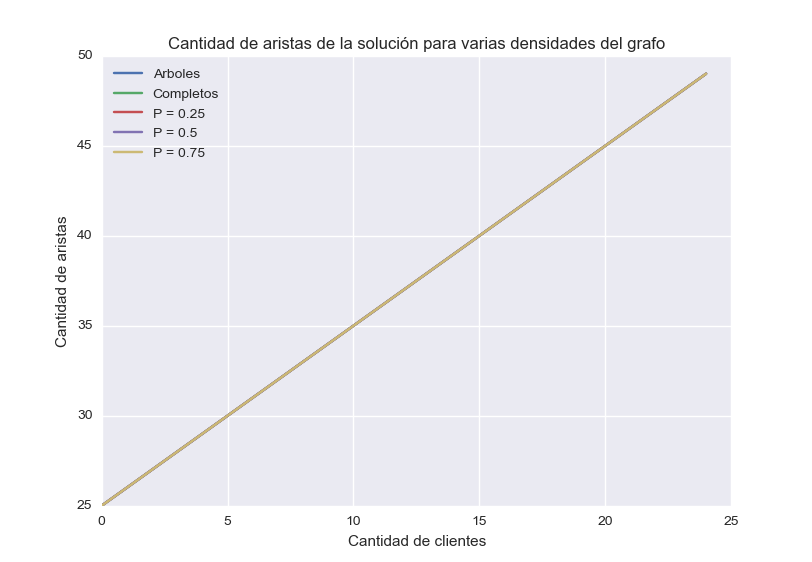
\includegraphics[width=0.6\textwidth]{tamanosolucion.png}
    \caption{La cantidad de aristas de la solución es igual a la cantidad de clientes para todos los casos analizados.}
    \label{fig:tamanosolucion}
\end{figure}

\newpage

El experimento se realizó dos veces, una con 50 casos de test de cada característica (con resultados promediados) y otra con uno solo, y los resultados fueron idénticos. Esto nos lleva a suponer que una solución óptima \textbf{sólo} puede tener una cantidad de aristas igual al número de clientes, y no que simplemente en la mayoría de los casos dio así. Por supuesto que la manera de probar que eso es verdad sería con una demostración formal, pero en base a este experimento, \textbf{hay evidencia muy fuerte para pensar que vale}.

Esta información también puede usarse para verificar la conjetura de que la cantidad de componentes conexas no puede superar a \textit{F}. Por una propiedad vista en la materia, un bosque con \textit{n} vértices y \textit{k} componentes conexas tiene exactamente \textit{n-k} aristas (en particular, un árbol tiene $n-1$). Entonces, si nuestros bosques tienen $F+C$ vértices y $C$ aristas, la cantidad de componentes conexas debería ser $F+C-C$, que es justamente \textit{F}. Entonces, si es verdad que toda solución tiene \textit{C} aristas, deducimos que también tiene \textbf{exactamente} \textit{F} componentes conexas.


\subsection{Experimento 6}

Dado que el algoritmo desarrollado está fuertemente basado en el algoritmo de Kruskal, el término dominante en su complejidad es el \textit{sort} de las aristas. Es interesante evaluar si el tiempo de ejecución también varía en función de la proporción de clientes a fábricas.

Antes de analizar cuidadosamente el algoritmo, podría parecer que una mayor proporción de clientes resultaría en un tiempo de ejecución mayor, puesto que la solución debe tener más aristas. Sin embargo, el ciclo -al igual que el de Kruskal clásico- itera una cantidad \textbf{fija} de veces (una vez por cada arista). Si una arista no puede ser agregada a la solución, simplemente pasa a la siguiente, y no tiene ninguna información que le indique si todas las aristas que le quedan por iterar son inútiles. Esto nos llevó a desarrollar esta hipótesis:

\paragraph{Hipótesis de proporción de clientes: } el tiempo de ejecución depende de la cantidad total de vértices y de la densidad del grafo, pero no de la proporción clientes/fábricas. Esto se debe a que el ciclo que arma la solución revisa todas las aristas, sin importar cuántas agregue.

\medskip

El primer conjunto de casos de test que elaboramos para poner a prueba esta hipótesis consiste en tres entradas con valores de \textit{F} y \textit{C} fijos: $F=10, C=20$, $F=20, C=30$ y $F=30, C=40$. Cada una de ellas contiene conjuntos de 80 casos en los que $p_a$ va desde 0.0 hasta 1.0 con intervalos de 0.05.

\begin{figure}[H]
    \centering
    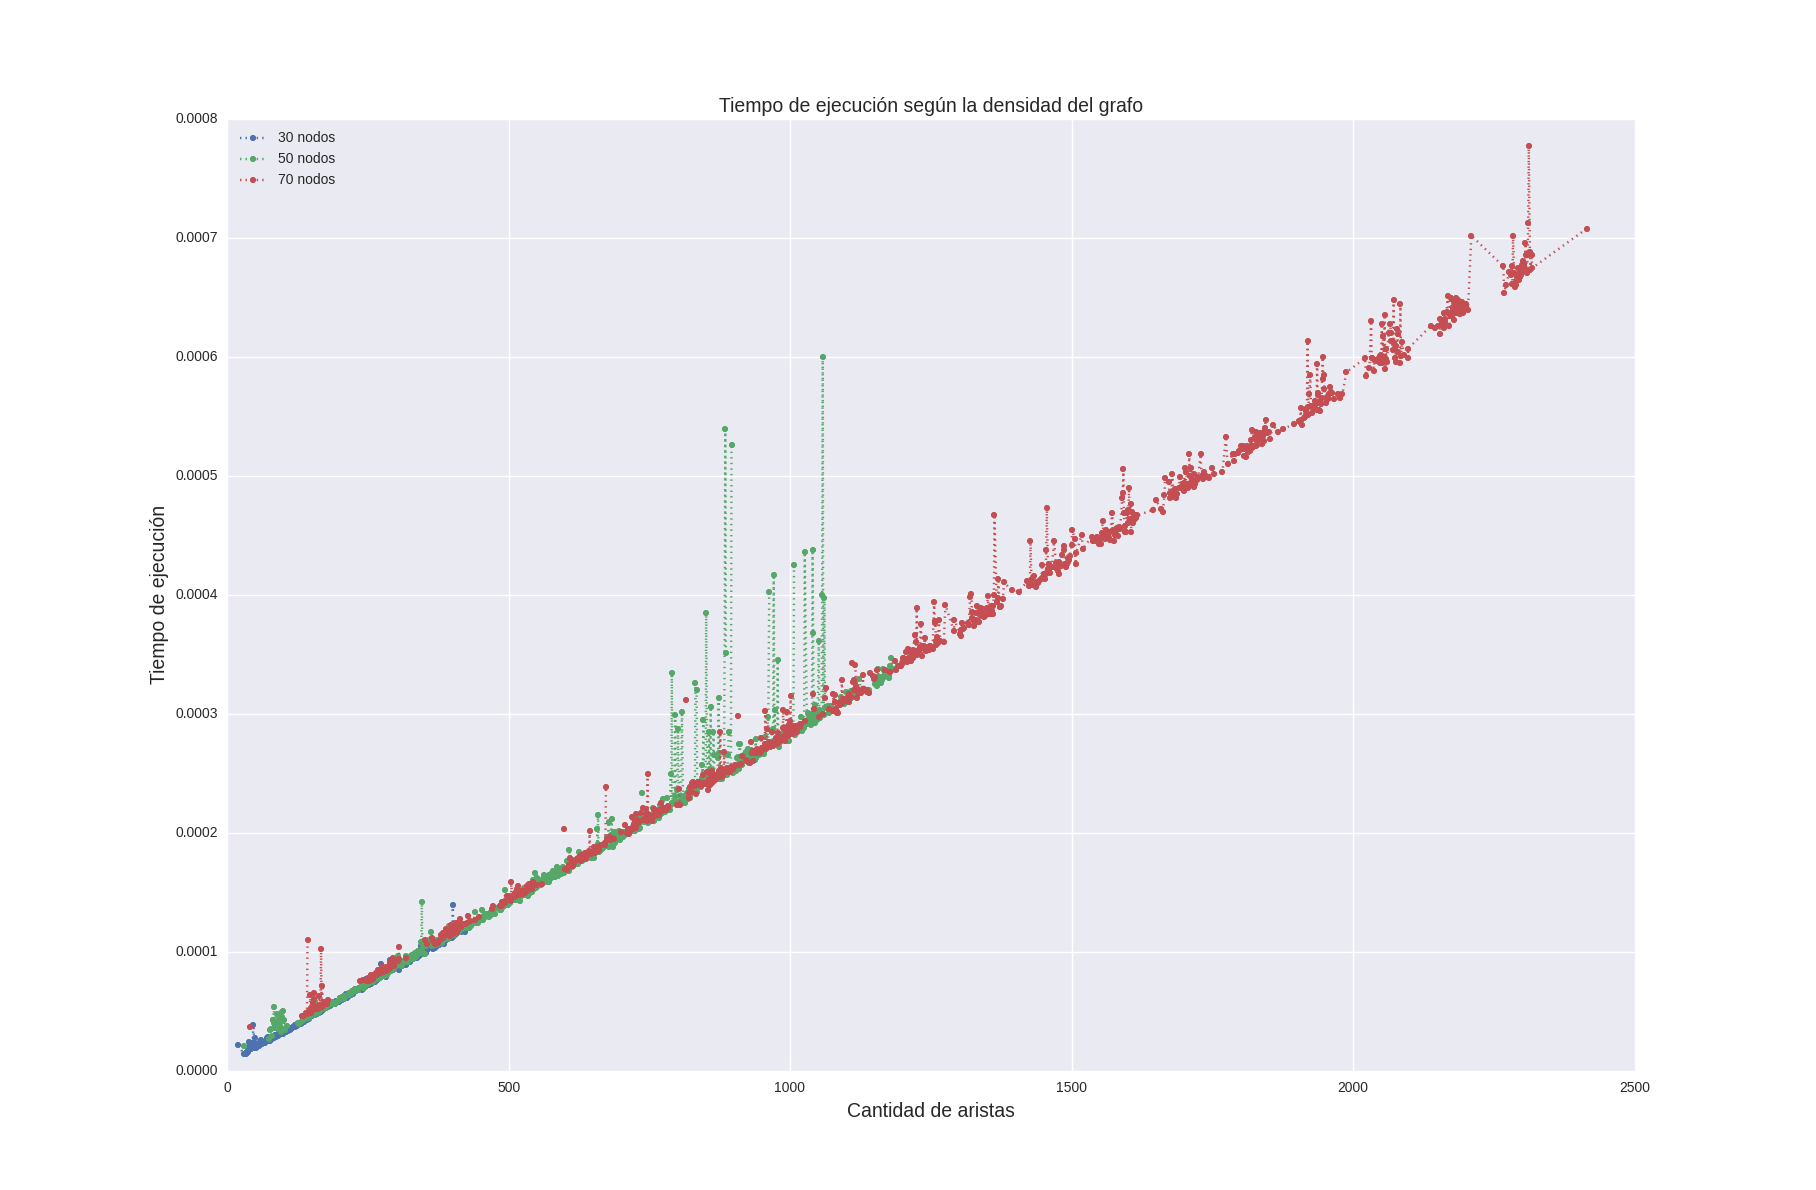
\includegraphics[width=\textwidth]{densidadcreciente.png}
    \caption{Tiempo de ejecución a medida que aumenta $E(R)$ para distintos valores fijos de $C$ y $F$.}
    \label{fig:densidadcreciente}
\end{figure}

\newpage

En el gráfico de la figura \ref{fig:densidadcreciente} podemos ver que el tiempo de ejecución efectivamente crece en función de $E(R)$. Además, más allá de las fluctuaciones \footnote{Es altamente probable que estas fluctuaciones se deban a \textit{outliers}, ya que como \textit{R} es una variable aleatoria, puede haber valores que se repitieron en muy pocos casos. Es debido a esto que no fue posible podar outliers.}, el ritmo de crecimiento se asemeja al de una \textbf{función lineal}. Considerando que \textit{C} está fijo en todos los casos de test, es esperable que el factor $log(C)$ de la complejidad teórica actúe como una \textbf{constante multiplicativa}, y la complejidad empírica para cada entrada sea similar a una función del tipo $f(R) = kR$.

Vale destacar que la proporción de clientes en cada una de estas entradas es respectivamente 0.66, 0.6 y 0.57; por más que la variación es poca, no es la misma en todas las entradas. Aun así, los tres gráficos son muy cercanos más allá de los \textit{outliers}. No consideramos que esta variación en $\frac{C}{F+C}$ sea suficiente para concluir que la proporción de clientes no tiene efectos observables en el tiempo de ejecución, por lo que elaboramos otro conjunto de casos de test en los que hay más variación.

El segundo conjunto consiste en 5 entradas con 50 vértices cada una en las que \textit{C} varía entre 25 y 49. En cada una, $p_a$ toma un valor distinto entre 0.0 y 1.0 con intervalos de 0.25. Como podemos ver en el gráfico de la figura \ref{fig:ccreciente}, el valor de \textit{C} \textbf{no tuvo efectos observables} en el tiempo de ejecución del algoritmo; la complejidad parece ser constante, más allá de fluctuaciones adjudicables a ruido externo. $p_a$, por el contrario, sí tuvo un efecto notable: las curvas están espaciadas de manera \textbf{directamente proporcional} a los valores de $E(R)$. Esto se condice con la similitud entre las curvas del gráfico anterior y las de una función lineal. En base a estos resultados, podemos concluir que hay evidencia fuerte \textbf{a favor} de la hipótesis de proporción de clientes.

\begin{figure}[!h]
    \centering
    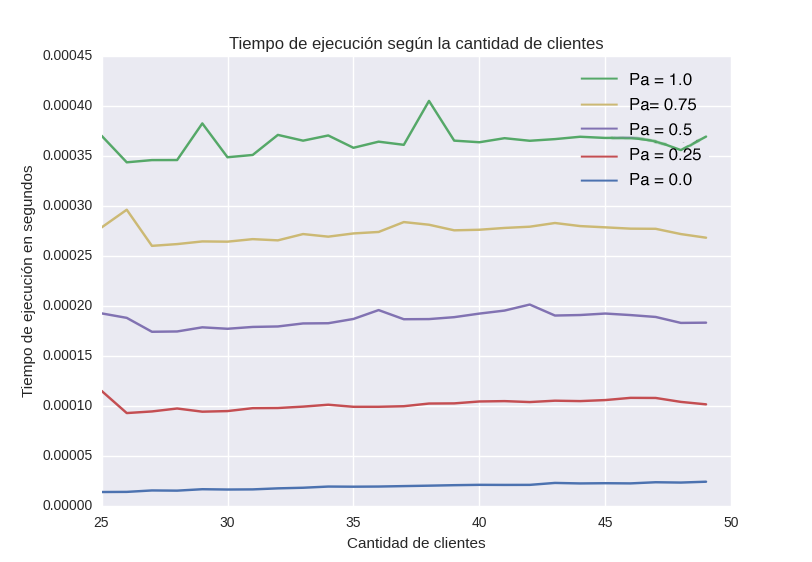
\includegraphics[width=0.75\textwidth]{ccreciente.png}
    \caption{Tiempo de ejecución a medida que \textit{C} aumenta, para distintos valores de $E(R)$}
    \label{fig:ccreciente}
\end{figure}

\subsection{Experimento 7}

En una sección anterior, argumentamos que la complejidad de este algoritmo, debido a las particularidades del problema a resolver, es $\mathcal{O}(Rlog(C))$, a pesar de que en un primer análisis sea $\mathcal{O}(Rlog(R))$. En este experimento, nos planteamos verificar si esto se refleja en la empiria o si se apoya en una propiedad teórica demasiado abstracta.

Para esto, generamos una entrada con casos de entre 5 y 20 clientes y la cantidad de fábricas fija en 5 (es decir, entre 10 y 25 vértices). A su vez, para cada cantidad de clientes, hicimos variar $p_a$ entre 0.0 y 1.0, con intervalos de 0.01. Para cada combinación de \textit{C} y $p_{a}$, generamos 80 casos de test. Posteriormente medimos la correlación entre los tiempos de ejecución de estos casos de test y la función $Rlog(C)$ evaluada en los mismos valores de \textit{F}, \textit{C} y \textit{R} (esta última variable es aleatoria en los casos de test, pero la consideramos que cantidad de muestras fue lo suficientemente grande como para compararla con los valores teóricos sin perder representatividad).

\begin{figure}[!h]
    \centering
    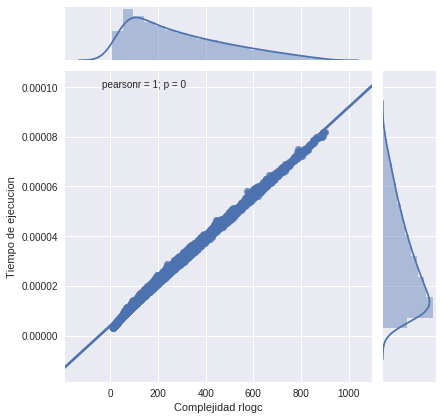
\includegraphics[width=0.65\textwidth]{pearsonRlogc.png}
    \caption{Correlación entre tiempos de ejecución empíricos y complejidad teórica}
    \label{fig:pearsonrlogc}
\end{figure}

En el gráfico de la figura \ref{fig:pearsonrlogc} podemos ver que el coeficiente de correlación de Pearson para la complejidad empírica y la teórica es 1, lo cual es \textbf{evidencia muy fuerte a favor de este postulado}. Este resultado es interesante, ya que muestra que este es un caso en el que usar el álgebra de órdenes de complejidad para deshacerse de las constantes refleja propiamente la complejidad del algoritmo en la práctica. En casos con constantes multiplicativas mayores, esto podría no ser así.

\end{document}
